\chap{空间中的四元数}
\section{介绍}
在本章中,我们将展示如何使用四元数来围绕任意轴旋转向量。我们首先回顾了一些与四元数相关的历史,特别是本杰明·奥林德·罗德里格斯(Benjamin Olinde Rodrigues)的作用,他发现了旋转变换中半角的重要性。

对于特定的四元数积,当四元数表示为
$$
q=[\cos \theta, \sin \theta \mathbf{v}]
$$

一个向量围绕轴$\mathbf{v}$旋转一个角度$\theta$。但是,我们会发现,对于三重四元数的乘积,当四元数表示为
$$
q=\left[\cos \frac{1}{2} \theta, \sin \frac{1}{2} \theta \mathbf{v}\right]
$$

一个向量围绕轴$\mathbf{v}$旋转一个角度$\theta$。这种半角表示是罗德里格斯发现的。

关于组合代数的简短部分揭示了四元数是相当特殊的,并告诉我们为什么 Hamilton 不能识别基于超复数$z=s+ i+ bj $的代数。

然后,我们检查了各种四元数乘积,以发现它们的旋转性质。这从两个正交四元数开始,然后转向使用三重$q p q^{-1}$的一般情况,其中$q$是一个单位范数四元数,$p$是一个纯四元数。

本章介绍了两种将四元数乘积表示为矩阵的方法,这两种方法依次编码特征向量和特征值。最后,我们研究如何插值四元数。

我们继续将四元数表示为有序对,用斜体小写字母表示四元数,用粗体小写字母表示向量。

\section{一点历史}
本杰明·罗德里格斯(Benjamin Olinde Rodrigues, 1795-1851)出生于法国波尔多。他在巴黎学习,并于1816年获得博士学位,时年21岁。他论文的主题是求解 Legendre 多项式, Rodrigues 提出了一个解,这个解至今仍被称为 Rodrigues 公式。

虽然他从事政治和银行业,但他的博士研究证实他不仅仅是一个“娱乐”数学家,因为在1840年,他在《纯数学年鉴》(Annales de Mathématiques Pures et Appliquées)上发表了一篇关于变换群[20]的数学论文。该文包含了一个公式,其描述了一个几何结构,即两个连续的围绕不同的轴的旋转,等价于第三个围绕另一个轴的旋转。今天,我们知道这种对应称为Euler-Rodrigues参数化。欧拉在1775年已经证明了一次旋转可以表示围绕不同轴的两次连续旋转,但没有提供代数解。

如果我们将一个关于轴向量$\mathbf{a}$的旋转$\alpha$表示为$\mathbf{R}_{\alpha, \mathbf{a}}$,那么Rodrigues提供了一个解决方案
$$
\mathbf{R}_{\gamma, \mathbf{n}}=\mathbf{R}_{\alpha, \mathbf{l}} \mathbf{R}_{\beta, \mathbf{m}}
$$

形式为
\begin{align}
& \cos \frac{1}{2} \gamma=\cos \frac{1}{2} \alpha \cos \frac{1}{2} \beta-\sin \frac{1}{2} \alpha \sin \frac{1}{2} \beta \mathbf{l} \cdot \mathbf{m} \\
& \sin \frac{1}{2} \gamma \mathbf{n}=\sin \frac{1}{2} \alpha \cos \frac{1}{2} \beta \mathbf{l}+\cos \frac{1}{2} \alpha \sin \frac{1}{2} \beta \mathbf{m}+\sin \frac{1}{2} \alpha \sin \frac{1}{2} \beta \mathbf{l} \times \mathbf{m} .
\end{align}

Rodrigues没有使用(7.1)和(7.2)中使用的向量符号,因为这还没有被Hamilton定义,但他确实使用了这些向量积的代数等价物。图$7.1$显示了罗德里格斯使用的由轴和旋转角组成的球形三角形。

\begin{figure}[h!]
    \centering
    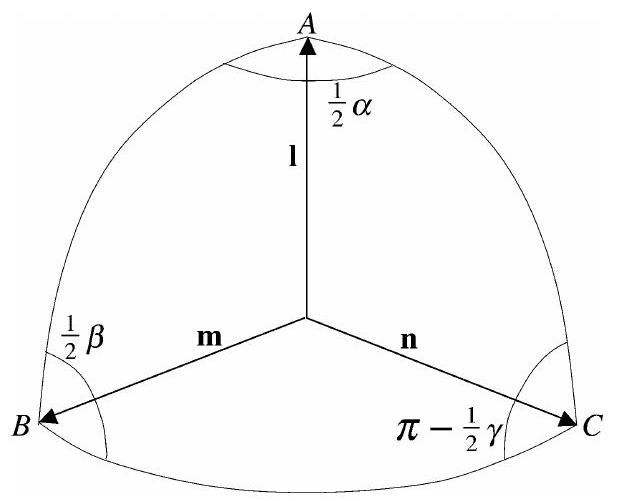
\includegraphics[max width=0.5\textwidth]{2023_01_16_a848224efad29cd66460g-105}
    \caption[short]{显示$\mathbf{l}$、$\mathbf{m}$和$\mathbf{n}$的Rodrigues球面三角形}
\end{figure}

式(7.1)和式(7.2)包含了一些四元数乘积所熟悉的特征,这些特征在下面的分析中变得很明显。我们从定义四元数开始

$$
\begin{aligned}
q_{l} & =\left[\cos \frac{1}{2} \alpha, \sin \frac{1}{2} \alpha \mathbf{l}\right] \\
q_{m} & =\left[\cos \frac{1}{2} \beta, \sin \frac{1}{2} \beta \mathbf{m}\right] \\
q_{n} & =\left[\cos \frac{1}{2} \gamma, \sin \frac{1}{2} \gamma \mathbf{n}\right]
\end{aligned}
$$

且乘积形式为
\begin{align}
q_{n}  =& q_{l} q_{m} \notag\\
=& \left[\cos \frac{1}{2} \alpha, \sin \frac{1}{2} \alpha \mathbf{l}\right]\left[\cos \frac{1}{2} \beta, \sin \frac{1}{2} \beta \mathbf{m}\right] \notag\\
=& \left[\cos \frac{1}{2} \alpha \cos \frac{1}{2} \beta-\sin \frac{1}{2} \alpha \sin \frac{1}{2} \beta \mathbf{l} \cdot \mathbf{m},\right. \notag\\
& \left.\sin \frac{1}{2} \alpha \cos \frac{1}{2} \beta \mathbf{l}+\cos \frac{1}{2} \alpha \sin \frac{1}{2} \beta \mathbf{m}+\sin \frac{1}{2} \alpha \sin \frac{1}{2} \beta \mathbf{l} \times \mathbf{m}\right] \notag\\
\cos \frac{1}{2} \gamma = & \cos \frac{1}{2} \alpha \cos \frac{1}{2} \beta-\sin \frac{1}{2} \alpha \sin \frac{1}{2} \beta \mathbf{l} \cdot \mathbf{m} \\
\sin \frac{1}{2} \gamma \mathbf{n} =& \sin \frac{1}{2} \alpha \cos \frac{1}{2} \beta \mathbf{l}+\cos \frac{1}{2} \alpha \sin \frac{1}{2} \beta \mathbf{m}+\sin \frac{1}{2} \alpha \sin \frac{1}{2} \beta \mathbf{l} \times \mathbf{m}
\end{align}

其中(7.3)和(7.4)分别与(7.1)和(7.2)相同。虽然Rodrigues没有发明四元数的形式
$$
q=s+a i+b j+c k,
$$

他在 Hamilton 之前就发现了四元数积的系数。这就是生活!\footnote{译注,法语:C'est la vie!}

Hamilton 在1843年10月发明了四元数,同年12月,他的朋友、爱尔兰数学家约翰·托马斯·格雷夫斯(John Thomas Graves, 1806-1870)发明了八度音阶,最终被称为八元数。英国数学家亚瑟·凯利(Arthur Cayley, 1821-1895)也对 Hamilton 的四元数很感兴趣,并于1845年独立发明了八元数。八元数最终被称为Cayley数而不是八元数,只是因为Graves直到1848年才发表了他的结果——比Cayley晚了3年!

正如四元数可以用复数的有序对来定义一样,八度或八元数也可以用四元数的有序对来定义。

\subsection{组合代数}
当一个特定的定律构成一个代数的基础时,它被称为组合代数。例如,我们知道在普通算术中
$$
a^{2} b^{2}=(a b)^{2} \qquad a, b \in \mathbb{R}
$$
比如
$$
3^{2} 4^{2}=12^{2}
$$
其中平方定律就是组合定律。

我们在第四章中发现,对于两个复数:
$$
\begin{aligned}
\left|z_{1}\right|\left|z_{2}\right| & =\left|z_{1} z_{2}\right| \qquad z_{1}, z_{2} \in \mathbb{C} \\
\left|z_{1}\right|^{2}\left|z_{2}\right|^{2} & =\left|z_{1} z_{2}\right|^{2} .
\end{aligned}
$$
举个例子, 给出
$$
\begin{aligned}
& z_{1}=a_{1}+b_{1} i \\
& z_{2}=a_{2}+b_{2} i
\end{aligned}
$$
然后
$$
\left(a_{1}^{2}+b_{1}^{2}\right)\left(a_{2}^{2}+b_{2}^{2}\right)=\left(a_{1} a_{2}-b_{1} b_{2}\right)^{2}+\left(a_{1} b_{2}+a_{2} b_{1}\right)^{2}
$$
这是一个2平方定律。

在第5章中,我们注意到对于两个四元数:
$$
\left|q_{a}\right|^{2}\left|q_{b}\right|^{2}=\left|q_{a} q_{b}\right|^{2} \quad q_{a}, q_{b} \in \mathbb{H} .
$$
举个例子, 给出
$$
\begin{aligned}
q_{a} & =\left[s_{a}, x_{a} \mathbf{i}+y_{a} \mathbf{j}+z_{a} \mathbf{k}\right] \\
q_{b} & =\left[s_{b}, x_{b} \mathbf{i}+y_{b} \mathbf{j}+z_{b} \mathbf{k}\right]
\end{aligned}
$$
然后
$$
\begin{aligned}
\left(s_{a}^{2}+x_{a}^{2}+y_{a}^{2}+z_{a}^{2}\right)\left(s_{b}^{2}+x_{b}^{2}+y_{b}^{2}+z_{b}^{2}\right)= & \left(s_{a} s_{b}-x_{a} x_{b}-y_{a} y_{b}-z_{a} z_{b}\right)^{2} \\
& +\left(s_{a} x_{b}+s_{b} x_{a}+y_{a} z_{b}-y_{b} z_{a}\right)^{2} \\
& +\left(s_{a} y_{b}+s_{b} y_{a}+z_{a} x_{b}-z_{b} x_{a}\right)^{2} \\
& +\left(s_{a} z_{b}+s_{b} z_{a}+x_{a} y_{b}-x_{b} y_{a}\right)^{2}
\end{aligned}
$$
这是四方定律。

除了复数,四元数在数学系统中占据着中心位置,今天有四个这样的组合代数:实$\mathbb{R}$、复$\mathbb{C}$、四元数$\mathbb{H}$和八元数$\mathbb{O}$,它们遵循$n$-平方的恒等式来计算它们的规范。1898年,德国数学家阿道夫·赫维茨(Adolf Hurwitz, 1859-1919)证明,只有当$n$等于1、2、4和8时,$n$的平方和与$n$的平方和的乘积才等于$n$的平方和,其中$n$用实数、复数、四元数和八元数表示。这就是所谓的“赫维茨定理”或“1,2,4,8定理”。没有其他系统是可能的,这表明四元数在数学领域是多么重要。因此,Hamilton对三元体系的探索是徒劳的,因为不存在三平方恒等式。

现在让我们研究如何使用四元数来围绕任意轴旋转向量。

\section{四元数乘积}
四元数$q$是标量$s$和向量$\mathbf{v}$的并集:
$$
q=[s, \mathbf{v}] \quad s \in \mathbb{R}, \mathbf{v} \in \mathbb{R}^{3}
$$

如果我们用$\mathbf{v}$的分量来表示它,我们有
$$
q=[s, x \mathbf{i}+y \mathbf{j}+z \mathbf{k}] \quad s, x, y, z \in \mathbb{R} .
$$

Hamilton曾希望四元数可以像复数转子一样使用,后者我们在第二章中看到了
$$
\mathbf{R}_{\theta}=\cos \theta+i \sin \theta
$$

将一个复数旋转$\theta$。单位范数四元数$q$可以用来旋转存储为纯四元数$p$的向量吗?是的,但只是在有限的意义上。为了理解这一点,让我们构造一个单位范数四元数$q$和一个纯四元数$p$的乘积。单位范数四元数$q$定义为
\begin{align}
\begin{aligned}
q & =[s, \lambda \hat{\mathbf{v}}] \quad s, \lambda \in \mathbb{R}, \hat{\mathbf{v}} \in \mathbb{R}^{3} \\
|\hat{\mathbf{v}}| & =1 \\
s^{2}+\lambda^{2} & =1
\end{aligned}
\end{align}
纯四元数$p$存储要旋转的向量$\mathbf{p}$:
$$
p=[0, \mathbf{p}] \quad \mathbf{p} \in \mathbb{R}^{3} .
$$

让我们计算乘积$p^{\prime}=q p$,并检查$p^{\prime}$的向量部分,看看$ \mathbf{p}$是否被旋转:
\begin{align}
\begin{aligned}
p^{\prime} & =q p \\
& =[s, \lambda \hat{\mathbf{v}}][0, \mathbf{p}] \\
& =[-\lambda \hat{\mathbf{v}} \cdot \mathbf{p}, s \mathbf{p}+\lambda \hat{\mathbf{v}} \times \mathbf{p}] .
\end{aligned}
\end{align}

我们可以从(7.6)中看到,结果是一个具有标量和向量分量的一般四元数。

\subsection{特殊情况}
上面提到的“狭义”是$\hat{\mathbf{v}}$必须垂直于$\mathbf{p}$,这使得点积项$-\lambda \hat{\mathbf{v}} \cdot \mathbf{p}$在(7.6)中消失,我们只剩下纯四元数

The 'restricted sense' referred to above is that $\hat{\mathbf{v}}$ must be perpendicular to $\mathbf{p}$, which makes the dot product term $-\lambda \hat{\mathbf{v}} \cdot \mathbf{p}$ in (7.6) vanish, and we are left with the pure quaternion

$$
p^{\prime}=[0, s \mathbf{p}+\lambda \hat{\mathbf{v}} \times \mathbf{p}] .
$$

Figure $7.2$ illustrates this scenario, where $\mathbf{p}$ is perpendicular to $\hat{\mathbf{v}}$, and $\hat{\mathbf{v}} \times \mathbf{p}$ is perpendicular to the plane containing $\mathbf{p}$ and $\hat{\mathbf{v}}$. Now because $\hat{\mathbf{v}}$ is a unit vector, $|\mathbf{p}|=|\hat{\mathbf{v}} \times \mathbf{p}|$, which means that we have two orthogonal vectors, i.e. $\mathbf{p}$ and $\hat{\mathbf{v}} \times \mathbf{p}$, with the same length. Therefore, to rotate $\mathbf{p}$ about $\hat{\mathbf{v}}$, all that we have to do is make $s=\cos \theta$ and $\lambda=\sin \theta$ in (7.7):

Fig. 7.2 Three orthogonal vectors $\mathbf{p}, \hat{\mathbf{v}}$ and $\hat{\mathbf{v}} \times \mathbf{p}$

Fig. 7.3 The vector $2 \mathbf{i}$ is rotated $45^{\circ}$ by the quaternion $q=\left[\frac{\sqrt{2}}{2}, \frac{\sqrt{2}}{2} \mathbf{k}\right]$
\begin{figure}
    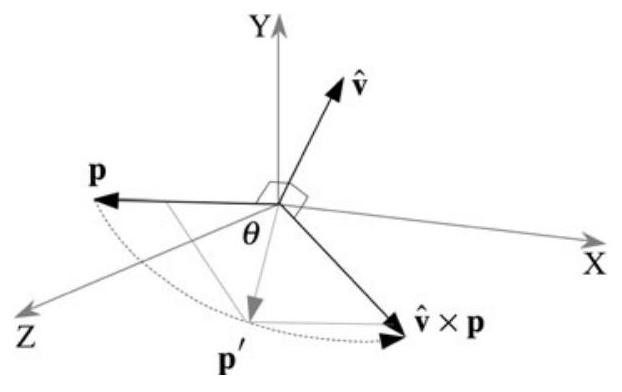
\includegraphics[max width=0.5\textwidth, center]{2023_01_16_a848224efad29cd66460g-109}
    \caption[short]{title}
\end{figure}




$$
\begin{aligned}
p^{\prime} & =\left[0, \mathbf{p}^{\prime}\right] \\
& =[0, \cos \theta \mathbf{p}+\sin \theta \hat{\mathbf{v}} \times \mathbf{p}]
\end{aligned}
$$

For example, to rotate a vector about the $z$-axis, $q$ 's vector $\hat{\mathbf{v}}$ must be aligned with the $z$-axis as shown in Fig. 7.3. If we make the angle of rotation $\theta=45^{\circ}$ then

$$
\begin{aligned}
q & =[s, \lambda \hat{\mathbf{v}}] \\
& =[\cos \theta, \sin \theta \mathbf{k}] \\
& =\left[\frac{\sqrt{2}}{2}, \frac{\sqrt{2}}{2} \mathbf{k}\right]
\end{aligned}
$$

and if the vector to be rotated is $\mathbf{p}=2 \mathbf{i}$, then

$$
\begin{aligned}
p & =[0, \mathbf{p}] \\
& =[0,2 \mathbf{i}] .
\end{aligned}
$$

There are now four product combinations worth exploring: $q p, p q, q^{-1} p$ and $p q^{-1}$. It's not worth considering $q p^{-1}$ and $p^{-1} q$ as $p^{-1}$ simply reverses the direction of $\mathbf{p}$. Let's start with $q p$ :

$$
\begin{aligned}
p^{\prime} & =q p \\
& =\left[\frac{\sqrt{2}}{2}, \frac{\sqrt{2}}{2} \mathbf{k}\right][0,2 \mathbf{i}] \\
& =\left[0,2 \frac{\sqrt{2}}{2} \mathbf{i}+2 \frac{\sqrt{2}}{2} \mathbf{k} \times \mathbf{i}\right] \\
& =[0, \sqrt{2} \mathbf{i}+\sqrt{2} \mathbf{j}]
\end{aligned}
$$

and $\mathbf{p}$ has been rotated $45^{\circ}$ to $\mathbf{p}^{\prime}=\sqrt{2} \mathbf{i}+\sqrt{2} \mathbf{j}$.

Next, $p q$ :

$$
\begin{aligned}
p^{\prime} & =p q \\
& =[0,2 \mathbf{i}]\left[\frac{\sqrt{2}}{2}, \frac{\sqrt{2}}{2} \mathbf{k}\right] \\
& =\left[0,2 \frac{\sqrt{2}}{2} \mathbf{i}-2 \frac{\sqrt{2}}{2} \mathbf{k} \times \mathbf{i}\right] \\
& =[0, \sqrt{2} \mathbf{i}-\sqrt{2} \mathbf{j}]
\end{aligned}
$$

and $\mathbf{p}$ has been rotated $-45^{\circ}$ to $\mathbf{p}^{\prime}=\sqrt{2} \mathbf{i}-\sqrt{2} \mathbf{j}$.

Next, $q^{-1} p$, and as $q$ is a unit-norm quaternion, $q^{-1}=q^{*}$ :

$$
\begin{aligned}
p^{\prime} & =q^{-1} p \\
& =\left[\frac{\sqrt{2}}{2},-\frac{\sqrt{2}}{2} \mathbf{k}\right][0,2 \mathbf{i}] \\
& =\left[0,2 \frac{\sqrt{2}}{2} \mathbf{i}-2 \frac{\sqrt{2}}{2} \mathbf{k} \times \mathbf{i}\right] \\
& =[0, \sqrt{2} \mathbf{i}-\sqrt{2} \mathbf{j}]
\end{aligned}
$$

and $\mathbf{p}$ has been rotated $-45^{\circ}$ to $\mathbf{p}^{\prime}=\sqrt{2} \mathbf{i}-\sqrt{2} \mathbf{j}$.

Finally, $p q^{-1}$ :

$$
\begin{aligned}
p^{\prime} & =p q^{-1} \\
& =[0,2 \mathbf{i}]\left[\frac{\sqrt{2}}{2},-\frac{\sqrt{2}}{2} \mathbf{k}\right] \\
& =\left[0,2 \frac{\sqrt{2}}{2} \mathbf{i}+2 \frac{\sqrt{2}}{2} \mathbf{k} \times \mathbf{i}\right] \\
& =[0, \sqrt{2} \mathbf{i}+\sqrt{2} \mathbf{j}]
\end{aligned}
$$

and $\mathbf{p}$ has been rotated $45^{\circ}$ to $\mathbf{p}^{\prime}=\sqrt{2} \mathbf{i}+\sqrt{2} \mathbf{j}$. Thus, for orthogonal quaternions, $\theta$ is the angle of rotation, then

$$
\begin{aligned}
& q p=p q^{-1} \\
& p q=q^{-1} p
\end{aligned}
$$

Fig. 7.4 Rotating the vector $\mathbf{p}=2 \mathbf{i}$ by the quaternion $q=[\cos \theta, \sin \theta \hat{\mathbf{v}}]$

\begin{center}
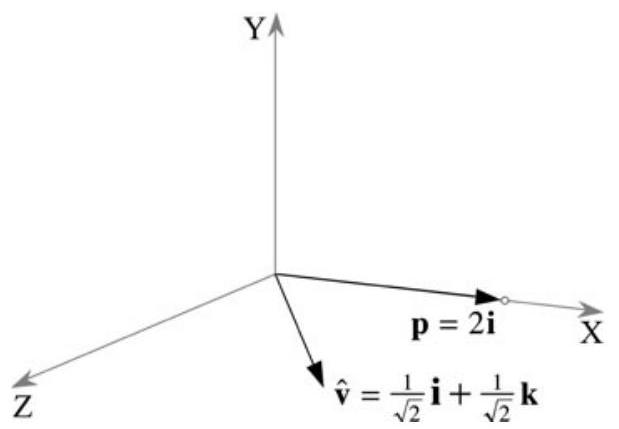
\includegraphics[max width=\textwidth]{2023_01_16_a848224efad29cd66460g-111}
\end{center}

Before moving on, let's see what happens to the product $q p$ when $\theta=180^{\circ}$ :

$$
\begin{aligned}
p^{\prime} & =q p \\
& =[-1, \mathbf{0}][0,2 \mathbf{i}] \\
& =[0,-2 \mathbf{i}]
\end{aligned}
$$

and $\mathbf{p}$ has been rotated $180^{\circ}$ to $\mathbf{p}^{\prime}=-2 \mathbf{i}$.

Note that in all the above products, the vector has not been scaled during the rotation. This is because $q$ is a unit-norm quaternion. Now let's see what happens if we change the angle between $\hat{\mathbf{v}}$ and $\mathbf{p}$. Let's reduce the angle to $45^{\circ}$ and retain $q$ 's unit vector, as shown in Fig. 7.4. Therefore,

$$
\begin{aligned}
\hat{\mathbf{v}} & =\frac{1}{\sqrt{2}} \mathbf{i}+\frac{1}{\sqrt{2}} \mathbf{k} \\
q & =[\cos \theta, \sin \theta \hat{\mathbf{v}}] \\
p & =[0, \mathbf{p}] .
\end{aligned}
$$

This time we must include the dot product term $-\sin \theta \hat{\mathbf{v}} \cdot \mathbf{p}$, as it is no longer zero:

$$
\begin{aligned}
p^{\prime} & =q p \\
& =[\cos \theta, \sin \theta \hat{\mathbf{v}}][0, \mathbf{p}] \\
& =[-\sin \theta \hat{\mathbf{v}} \cdot \mathbf{p}, \cos \theta \mathbf{p}+\sin \theta \hat{\mathbf{v}} \times \mathbf{p}] .
\end{aligned}
$$

Substituting $\hat{\mathbf{v}}, \mathbf{p}$ and $\theta=45^{\circ}$ in $(7.8)$, we have

$$
\begin{aligned}
p^{\prime} & =\left[-\frac{\sqrt{2}}{2}\left(\frac{1}{\sqrt{2}} \mathbf{i}+\frac{1}{\sqrt{2}} \mathbf{k}\right) \cdot(2 \mathbf{i}), \frac{\sqrt{2}}{2} 2 \mathbf{i}+\frac{\sqrt{2}}{2}\left(\frac{1}{\sqrt{2}} \mathbf{i}+\frac{1}{\sqrt{2}} \mathbf{k}\right) \times 2 \mathbf{i}\right] \\
& =[-1, \sqrt{2} \mathbf{i}+\mathbf{j}]
\end{aligned}
$$

which, unfortunately, is no longer a pure quaternion. It has not been rotated $45^{\circ}$, and the vector's norm is reduced to $\sqrt{3}$ ! Multiplying the vector by a non-orthogonal quaternion has converted some of the vector information into the quaternion's scalar component. Fig. 7.5 The vector $2 \mathbf{i}$ is rotated $90^{\circ}$ to $\mathbf{i}+\sqrt{2} \mathbf{j}+\mathbf{k}$

\begin{center}
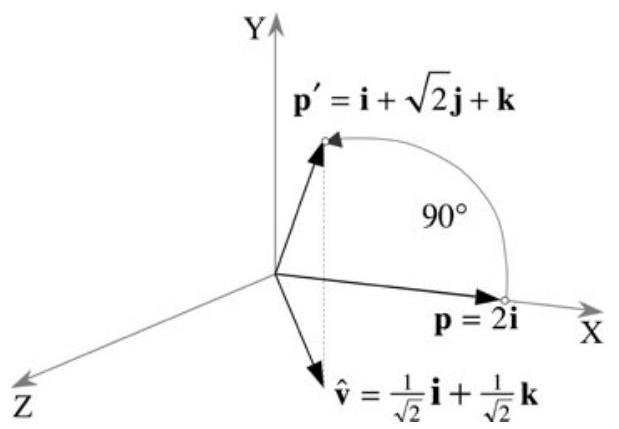
\includegraphics[max width=\textwidth]{2023_01_16_a848224efad29cd66460g-112}
\end{center}

\subsection{一般情况}
Not to worry. Could it be that an inverse quaternion reverses the operation? Let's see what happens if we post-multiply $q p$ by $q^{-1}$.

Given

$$
q=\left[\cos \theta, \sin \theta\left(\frac{1}{\sqrt{2}} \mathbf{i}+\frac{1}{\sqrt{2}} \mathbf{k}\right)\right]
$$

then

$$
\begin{aligned}
q^{-1} & =\left[\cos \theta,-\sin \theta\left(\frac{1}{\sqrt{2}} \mathbf{i}+\frac{1}{\sqrt{2}} \mathbf{k}\right)\right] \\
& =\left[\frac{\sqrt{2}}{2}, \frac{\sqrt{2}}{2}\left(\frac{1}{\sqrt{2}} \mathbf{i}+\frac{1}{\sqrt{2}} \mathbf{k}\right)\right] \\
& =\frac{1}{2}[\sqrt{2},-\mathbf{i}-\mathbf{k}] .
\end{aligned}
$$

Therefore, post-multiplying (7.9) by $q^{-1}$ we have

$$
\begin{aligned}
q p q^{-1} & =[-1, \sqrt{2} \mathbf{i}+\mathbf{j}] \frac{1}{2}[\sqrt{2},-\mathbf{i}-\mathbf{k}] \\
& =\frac{1}{2}[-\sqrt{2}-(\sqrt{2} \mathbf{i}+\mathbf{j}) \cdot(-\mathbf{i}-\mathbf{k}), \mathbf{i}+\mathbf{k}+\sqrt{2}(\sqrt{2} \mathbf{i}+\mathbf{j})-\mathbf{i}+\sqrt{2} \mathbf{j}+\mathbf{k}] \\
& =\frac{1}{2}[-\sqrt{2}+\sqrt{2}, \mathbf{i}+\mathbf{k}+2 \mathbf{i}+\sqrt{2} \mathbf{j}-\mathbf{i}+\sqrt{2} \mathbf{j}+\mathbf{k}] \\
& =[0, \mathbf{i}+\sqrt{2} \mathbf{j}+\mathbf{k}]
\end{aligned}
$$

which is a pure quaternion. Furthermore, there's no scaling as its norm is still 2, but the vector has been rotated $90^{\circ}$ rather than $45^{\circ}$, twice the desired angle, as shown in Fig. 7.5.

If this 'sandwiching' of the vector in the form of a pure quaternion by $q$ and $q^{-1}$ is correct, it suggests that increasing $\theta$ to $90^{\circ}$ should rotate $\mathbf{p}=2 \mathbf{i}$ by $180^{\circ}$ to $2 \mathbf{k}$. Let's try this. Let $\theta=90^{\circ}$, therefore,

$$
\begin{aligned}
q p & =\left[0, \frac{1}{\sqrt{2}} \mathbf{i}+\frac{1}{\sqrt{2}} \mathbf{k}\right][0,2 \mathbf{i}] \\
& =\left[-\frac{2}{\sqrt{2}}, \frac{2}{\sqrt{2}} \mathbf{j}\right]
\end{aligned}
$$

Next, we post-multiply $q p$ by $q^{-1}$ :

$$
\begin{aligned}
q u p q^{-1} & =\left[-\frac{2}{\sqrt{2}}, \frac{2}{\sqrt{2}} \mathbf{j}\right]\left[0,-\frac{1}{\sqrt{2}} \mathbf{i}-\frac{1}{\sqrt{2}} \mathbf{k}\right] \\
& =[0, \mathbf{i}+\mathbf{k}-\mathbf{i}+\mathbf{k}] \\
& =[0,2 \mathbf{k}]
\end{aligned}
$$

which confirms our prediction and suggests that $q p q^{-1}$ works. Now let's show how this double angle arises. We begin by defining a unit-norm quaternion $q$ :

$$
q=[s, \lambda \hat{\mathbf{v}}]
$$

where $s^{2}+\lambda^{2}=1$. The vector $\mathbf{p}$ to be rotated is encoded as a pure quaternion:

$$
p=[0, \mathbf{p}]
$$

and the inverse quaternion $q^{-1}$ is

$$
q^{-1}=[s,-\lambda \hat{\mathbf{v}}]
$$

Therefore, the product $q p q^{-1}$ is

$$
\begin{aligned}
q p q^{-1}= & {[s, \lambda \hat{\mathbf{v}}][0, \mathbf{p}][s,-\lambda \hat{\mathbf{v}}] } \\
= & {[-\lambda \hat{\mathbf{v}} \cdot \mathbf{p}, s \mathbf{p}+\lambda \hat{\mathbf{v}} \times \mathbf{p}][s,-\lambda \hat{\mathbf{v}}] } \\
= & {\left[-\lambda s \hat{\mathbf{v}} \cdot \mathbf{p}+\lambda s \mathbf{p} \cdot \hat{\mathbf{v}}+\lambda^{2}(\hat{\mathbf{v}} \times \mathbf{p}) \cdot \hat{\mathbf{v}}\right.} \\
& \lambda^{2}(\hat{\mathbf{v}} \cdot \mathbf{p}) \hat{\mathbf{v}}+s^{2} \mathbf{p}+\lambda s \hat{\mathbf{v}} \times \mathbf{p} \\
& \left.-\lambda s \mathbf{p} \times \hat{\mathbf{v}}-\lambda^{2}(\hat{\mathbf{v}} \times \mathbf{p}) \times \hat{\mathbf{v}}\right] \\
= & {\left[\lambda^{2}(\hat{\mathbf{v}} \times \mathbf{p}) \cdot \hat{\mathbf{v}}, \lambda^{2}(\hat{\mathbf{v}} \cdot \mathbf{p}) \hat{\mathbf{v}}+s^{2} \mathbf{p}+2 \lambda s \hat{\mathbf{v}} \times \mathbf{p}-\lambda^{2}(\hat{\mathbf{v}} \times \mathbf{p}) \times \hat{\mathbf{v}}\right] }
\end{aligned}
$$

Note that

$$
(\hat{\mathbf{v}} \times \mathbf{p}) \cdot \hat{\mathbf{v}}=0
$$

and

$$
(\hat{\mathbf{v}} \times \mathbf{p}) \times \hat{\mathbf{v}}=(\hat{\mathbf{v}} \cdot \hat{\mathbf{v}}) \mathbf{p}-(\mathbf{p} \cdot \hat{\mathbf{v}}) \hat{\mathbf{v}}=\mathbf{p}-(\mathbf{p} \cdot \hat{\mathbf{v}}) \hat{\mathbf{v}}
$$

Therefore,

$$
\begin{aligned}
q p q^{-1} & =\left[0, \lambda^{2}(\hat{\mathbf{v}} \cdot \mathbf{p}) \hat{\mathbf{v}}+s^{2} \mathbf{p}+2 \lambda s \hat{\mathbf{v}} \times \mathbf{p}-\lambda^{2} \mathbf{p}+\lambda^{2}(\mathbf{p} \cdot \hat{\mathbf{v}}) \hat{\mathbf{v}}\right] \\
& =\left[0,2 \lambda^{2}(\hat{\mathbf{v}} \cdot \mathbf{p}) \hat{\mathbf{v}}+\left(s^{2}-\lambda^{2}\right) \mathbf{p}+2 \lambda s \hat{\mathbf{v}} \times \mathbf{p}\right]
\end{aligned}
$$

Obviously, this is a pure quaternion as the scalar component is zero. However, it is not obvious where the angle doubling comes from. But look what happens when we make $s=\cos \theta$ and $\lambda=\sin \theta$ :

$$
\begin{aligned}
q p q^{-1} & =\left[0,2 \sin ^{2} \theta(\hat{\mathbf{v}} \cdot \mathbf{p}) \hat{\mathbf{v}}+\left(\cos ^{2} \theta-\sin ^{2} \theta\right) \mathbf{p}+2 \sin \theta \cos \theta \hat{\mathbf{v}} \times \mathbf{p}\right] \\
& =[0,(1-\cos 2 \theta)(\hat{\mathbf{v}} \cdot \mathbf{p}) \hat{\mathbf{v}}+\cos 2 \theta \mathbf{p}+\sin 2 \theta \hat{\mathbf{v}} \times \mathbf{p}] .
\end{aligned}
$$

The double-angle trigonometric terms emerge! Now, if we want this product to actually rotate the vector by $\theta$, then we must build this in from the outset by halving $\theta$ in $q$ :

$$
q=\left[\cos \frac{1}{2} \theta, \sin \frac{1}{2} \theta \hat{\mathbf{v}}\right]
$$

which makes

$$
q p q^{-1}=[0,(1-\cos \theta)(\hat{\mathbf{v}} \cdot \mathbf{p}) \hat{\mathbf{v}}+\cos \theta \mathbf{p}+\sin \theta \hat{\mathbf{v}} \times \mathbf{p}]
$$

The product $q p q^{-1}$ was discovered by Hamilton who failed to publish the result. Cayley, also discovered the product and published the result in 1845 [8]. However, Altmann notes that "in Cayley's collected papers he concedes priority to Hamilton" [2], which was a nice gesture. However, the person who had recognised the importance of the half-angle parameters in (7.12) before Hamilton and Cayley was Rodrigues-who published a solution that was not seen by Hamilton, but apparently, was seen by Cayley.

Let's test (7.13) using the previous example where we rotated a vector $\mathbf{p}=2 \mathbf{i}$, $\theta=90^{\circ}$ about the quaternion's vector $\hat{\mathbf{v}}=(1 / \sqrt{2}) \mathbf{i}+(1 / \sqrt{2}) \mathbf{k}$.

$$
\begin{aligned}
q u p q^{-1} & =[0,(1-\cos \theta)(\hat{\mathbf{v}} \cdot \mathbf{p}) \hat{\mathbf{v}}+\cos \theta \mathbf{p}+\sin \theta \hat{\mathbf{v}} \times \mathbf{p}] \\
& =[0,(\hat{\mathbf{v}} \cdot \mathbf{p}) \hat{\mathbf{v}}+\hat{\mathbf{v}} \times \mathbf{p}] \\
& =\left[0, \frac{2}{\sqrt{2}}\left(\frac{1}{\sqrt{2}} \mathbf{i}+\frac{1}{\sqrt{2}} \mathbf{k}\right)+\sqrt{2} \mathbf{j}\right] \\
& =[0, \mathbf{i}+\sqrt{2} \mathbf{j}+\mathbf{k}]
\end{aligned}
$$

which agrees with (7.10). Thus, when a unit-norm quaternion takes the form

$$
q=\left[\cos \frac{1}{2} \theta, \sin \frac{1}{2} \theta \hat{\mathbf{v}}\right]
$$

and a pure quaternion storing a vector to be rotated takes the form

$$
p=[0, \mathbf{p}]
$$

the pure quaternion

$$
p^{\prime}=q p q^{-1}
$$

stores the rotated vector $\mathbf{p}^{\prime}$. Let's show why this product preserves the magnitude of the rotated vector.

$$
\begin{aligned}
\left|p^{\prime}\right| & =|q p|\left|q^{-1}\right| \\
& =|q||p|\left|q^{-1}\right| \\
& =|q|^{2}|p|
\end{aligned}
$$

and if $q$ is a unit-norm quaternion, $|q|=1$, then $\left|p^{\prime}\right|=|p|$.

You may be wondering what happens if the product is reversed to $q^{-1} p q$ ? A guess would suggest that the rotation sequence is reversed, but let's see what an algebraic analysis confirms.

$$
\begin{aligned}
q^{-1} p q= & {[s,-\lambda \hat{\mathbf{v}}][0, \mathbf{p}][s, \lambda \hat{\mathbf{v}}] } \\
= & {[\lambda \hat{\mathbf{v}} \cdot \mathbf{p}, s \mathbf{p}-\lambda \hat{\mathbf{v}} \times \mathbf{p}][s, \lambda \hat{\mathbf{v}}] } \\
= & {[\lambda s \hat{\mathbf{v}} \cdot \mathbf{p}-\lambda s \mathbf{p} \cdot \hat{\mathbf{v}}} \\
& \left.\lambda^{2} \hat{\mathbf{v}} \times \mathbf{p} \cdot \hat{\mathbf{v}}+\lambda^{2} \hat{\mathbf{v}} \cdot \mathbf{p} \hat{\mathbf{v}}+s^{2} \mathbf{p}-\lambda s \hat{\mathbf{v}} \times \mathbf{p}+\lambda s \mathbf{p} \times \hat{\mathbf{v}}-\lambda^{2} \hat{\mathbf{v}} \times \mathbf{p} \times \hat{\mathbf{v}}\right] \\
= & {\left[\lambda^{2}(\hat{\mathbf{v}} \times \mathbf{p}) \cdot \hat{\mathbf{v}}, \lambda^{2}(\hat{\mathbf{v}} \cdot \mathbf{p}) \hat{\mathbf{v}}+s^{2} \mathbf{p}-2 \lambda s \hat{\mathbf{v}} \times \mathbf{p}-\lambda^{2}(\hat{\mathbf{v}} \times \mathbf{p}) \times \hat{\mathbf{v}}\right] }
\end{aligned}
$$

Once again

$$
(\hat{\mathbf{v}} \times \mathbf{p}) \cdot \hat{\mathbf{v}}=0
$$

and

$$
(\hat{\mathbf{v}} \times \mathbf{p}) \times \hat{\mathbf{v}}=\mathbf{p}-(\mathbf{p} \cdot \hat{\mathbf{v}}) \hat{\mathbf{v}}
$$

Therefore,

$$
\begin{aligned}
q^{-1} p q & =\left[0, \lambda^{2}(\hat{\mathbf{v}} \cdot \mathbf{p}) \hat{\mathbf{v}}+s^{2} \mathbf{p}-2 \lambda s \hat{\mathbf{v}} \times \mathbf{p}-\lambda^{2} \mathbf{p}+\lambda^{2}(\mathbf{p} \cdot \hat{\mathbf{v}}) \hat{\mathbf{v}}\right] \\
& =\left[0,2 \lambda^{2}(\hat{\mathbf{v}} \cdot \mathbf{p}) \hat{\mathbf{v}}+\left(s^{2}-\lambda^{2}\right) \mathbf{p}-2 \lambda s \hat{\mathbf{v}} \times \mathbf{p}\right]
\end{aligned}
$$

Again, let's make $s=\cos \theta$ and $\lambda=\sin \theta$ :

$$
q^{-1} p q=[0,(1-\cos 2 \theta)(\hat{\mathbf{v}} \cdot \mathbf{p}) \hat{\mathbf{v}}+\cos 2 \theta \mathbf{p}-\sin 2 \theta \hat{\mathbf{v}} \times \mathbf{p}]
$$

and the only thing that has changed from $q p q^{-1}$ is the sign of the cross-product term, which reverses the direction of its vector. However, we must remember to compensate for the angle-doubling by halving $\theta$ :

$$
q^{-1} p q=[0,(1-\cos \theta)(\hat{\mathbf{v}} \cdot \mathbf{p}) \hat{\mathbf{v}}+\cos \theta \mathbf{p}-\sin \theta \hat{\mathbf{v}} \times \mathbf{p}]
$$

Let's see what happens when we employ (7.14) to rotate $\mathbf{p}=2 \mathbf{i}, 90^{\circ}$ about the quaternion's vector $\hat{\mathbf{v}}=(1 / \sqrt{2}) \mathbf{i}+(1 / \sqrt{2}) \mathbf{k}$ :

$$
\begin{aligned}
q^{-1} p q & =\left[0, \frac{2}{\sqrt{2}}\left(\frac{1}{\sqrt{2}} \mathbf{i}+\frac{1}{\sqrt{2}} \mathbf{k}\right)-\sqrt{2} \mathbf{j}\right] \\
& =[0, \mathbf{i}-\sqrt{2} \mathbf{j}+\mathbf{k}]
\end{aligned}
$$

which has rotated $\mathbf{p}$ clockwise $90^{\circ}$ about the quaternion's vector. Therefore, the rotor $q p q^{-1}$ rotates a vector counter-clockwise, and $q^{-1} p q$ rotates a vector Fig. 7.6 The point $P(0,1,1)$ is rotated $90^{\circ}$ to $P^{\prime}(1,1,0)$ about the $y$-axis

\begin{center}
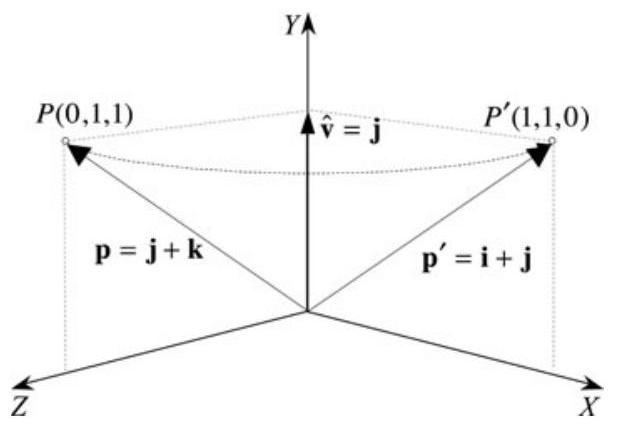
\includegraphics[max width=\textwidth]{2023_01_16_a848224efad29cd66460g-116}
\end{center}

clockwise:

$$
\begin{aligned}
q p q^{-1} & =[0,(1-\cos \theta)(\hat{\mathbf{v}} \cdot \mathbf{p}) \hat{\mathbf{v}}+\cos \theta \mathbf{p}+\sin \theta \hat{\mathbf{v}} \times \mathbf{p}] \\
q^{-1} p q & =[0,(1-\cos \theta)(\hat{\mathbf{v}} \cdot \mathbf{p}) \hat{\mathbf{v}}+\cos \theta \mathbf{p}-\sin \theta \hat{\mathbf{v}} \times \mathbf{p}]
\end{aligned}
$$

Let's compute another example. Consider the point $P(0,1,1)$ in Fig. $7.6$ which is to be rotated $90^{\circ}$ about the $y$-axis. We can see that the rotated point $P^{\prime}$ has the coordinates $(1,1,0)$ which we will confirm algebraically. The point $P$ is represented by its position vector $\mathbf{p}$ in the pure quaternion

$$
p=[0, \mathbf{p}] \text {. }
$$

The axis of rotation is $\hat{\mathbf{v}}=\mathbf{j}$, and the vector to be rotated is $\mathbf{p}=\mathbf{j}+\mathbf{k}$. Therefore,

$$
\begin{aligned}
\operatorname{qpq}^{-1} & =[0,(1-\cos \theta)(\hat{\mathbf{v}} \cdot \mathbf{p}) \hat{\mathbf{v}}+\cos \theta \mathbf{p}+\sin \theta \hat{\mathbf{v}} \times \mathbf{p}] \\
& =[0, \mathbf{j} \cdot(\mathbf{j}+\mathbf{k}) \mathbf{j}+\mathbf{j} \times(\mathbf{j}+\mathbf{k})] \\
& =[0, \mathbf{i}+\mathbf{j}]
\end{aligned}
$$

and confirms that $P$ is indeed rotated to $(1,1,0)$.

Now let's explore how this product is represented in matrix form.

\section{矩阵形式的四元数}
Having discovered a vector equation to represent the triple $q p q^{-1}$, let's continue and convert it into a matrix. We will explore two methods: the first is a simple vectorial method which translates the vector equation representing $q p q^{-1}$ directly into matrix form. The second method uses matrix algebra to develop a rather cunning solution.

\subsection{向量方法}
For the vector method it is convenient to describe the unit-norm quaternion as

$$
\begin{aligned}
q & =[s, \mathbf{v}] \\
& =[s, x \mathbf{i}+y \mathbf{j}+z \mathbf{k}]
\end{aligned}
$$

where

$$
s^{2}+|\mathbf{v}|^{2}=1
$$

and the pure quaternion as

$$
\begin{aligned}
p & =[0, \mathbf{p}] \\
& =\left[0, x_{p} \mathbf{i}+y_{p} \mathbf{j}+z_{p} \mathbf{k}\right] .
\end{aligned}
$$

A simple way to compute $q p q^{-1}$ is to use (7.11) and substitute $|\mathbf{v}|$ for $\lambda$ :

$$
\begin{aligned}
q p q^{-1} & =\left[0,2 \lambda^{2}(\hat{\mathbf{v}} \cdot \mathbf{p}) \hat{\mathbf{v}}+\left(s^{2}-\lambda^{2}\right) \mathbf{p}+2 \lambda s \hat{\mathbf{v}} \times \mathbf{p}\right] \\
& =\left[0,2|\mathbf{v}|^{2}(\hat{\mathbf{v}} \cdot \mathbf{p}) \hat{\mathbf{v}}+\left(s^{2}-|\mathbf{v}|^{2}\right) \mathbf{p}+2|\mathbf{v}| s \hat{\mathbf{v}} \times \mathbf{p}\right]
\end{aligned}
$$

Next, we substitute $\mathbf{v}$ for $|\mathbf{v}| \hat{\mathbf{v}}$ :

$$
q p q^{-1}=\left[0,2(\mathbf{v} \cdot \mathbf{p}) \mathbf{v}+\left(s^{2}-|\mathbf{v}|^{2}\right) \mathbf{p}+2 s \mathbf{v} \times \mathbf{p}\right]
$$

Finally, as we are working with unit-norm quaternions to prevent scaling

$$
s^{2}+|\mathbf{v}|^{2}=1
$$

and

$$
s^{2}-|\mathbf{v}|^{2}=2 s^{2}-1
$$

therefore,

$$
q p q^{-1}=\left[0,2(\mathbf{v} \cdot \mathbf{p}) \mathbf{v}+\left(2 s^{2}-1\right) \mathbf{p}+2 s \mathbf{v} \times \mathbf{p}\right]
$$

If we let $p^{\prime}=q p q^{-1}$, which is a pure quaternion, we have

$$
\begin{aligned}
p^{\prime} & =q p q^{-1} \\
& =\left[0, \mathbf{p}^{\prime}\right] \\
& =\left[0,2(\mathbf{v} \cdot \mathbf{p}) \mathbf{v}+\left(2 s^{2}-1\right) \mathbf{p}+2 s \mathbf{v} \times \mathbf{p}\right] \\
\mathbf{p}^{\prime} & =2(\mathbf{v} \cdot \mathbf{p}) \mathbf{v}+\left(2 s^{2}-1\right) \mathbf{p}+2 s \mathbf{v} \times \mathbf{p} .
\end{aligned}
$$

We are only interested in the rotated vector $\mathbf{p}^{\prime}$ comprising the three terms $2(\mathbf{v} \cdot \mathbf{p}) \mathbf{v}$, $\left(2 s^{2}-1\right) \mathbf{p}$ and $2 s \mathbf{v} \times \mathbf{p}$, which can be represented by three individual matrices and summed together.

$$
\begin{aligned}
2(\mathbf{v} \cdot \mathbf{p}) \mathbf{v} & =2\left(x x_{p}+y y_{p}+z z_{p}\right)(x \mathbf{i}+y \mathbf{j}+z \mathbf{k}) \\
& =\left[\begin{array}{lll}
2 x^{2} & 2 x y & 2 x z \\
2 x y & 2 y^{2} & 2 y z \\
2 x z & 2 y z & 2 z^{2}
\end{array}\right]\left[\begin{array}{l}
x_{p} \\
y_{p} \\
z_{p}
\end{array}\right] \\
\left(2 s^{2}-1\right) \mathbf{p} & =\left(2 s^{2}-1\right) x_{p} \mathbf{i}+\left(2 s^{2}-1\right) y_{p} \mathbf{j}+\left(2 s^{2}-1\right) z_{p} \mathbf{k} \\
& =\left[\begin{array}{ccc}
2 s^{2}-1 & 0 & 0 \\
0 & 2 s^{2}-1 & 0 \\
0 & 0 & 2 s^{2}-1
\end{array}\right]\left[\begin{array}{l}
x_{p} \\
y_{p} \\
z_{p}
\end{array}\right]
\end{aligned}
$$

$$
\begin{aligned}
2 s \mathbf{v} \times \mathbf{p} & =2 s\left(\left(y z_{p}-z y_{p}\right) \mathbf{i}+\left(z x_{p}-x z_{p}\right) \mathbf{j}+\left(x y_{p}-y x_{p}\right) \mathbf{k}\right) \\
& =\left[\begin{array}{ccc}
0 & -2 s z & 2 s y \\
2 s z & 0 & -2 s x \\
-2 s y & 2 s x & 0
\end{array}\right]\left[\begin{array}{l}
x_{p} \\
y_{p} \\
z_{p}
\end{array}\right] .
\end{aligned}
$$

Adding these matrices together:

$$
\mathbf{p}^{\prime}=\left[\begin{array}{ccc}
2\left(s^{2}+x^{2}\right)-1 & 2(x y-s z) & 2(x z+s y) \\
2(x y+s z) & 2\left(s^{2}+y^{2}\right)-1 & 2(y z-s x) \\
2(x z-s y) & 2(y z+s x) & 2\left(s^{2}+z^{2}\right)-1
\end{array}\right]\left[\begin{array}{l}
x_{p} \\
y_{p} \\
z_{p}
\end{array}\right]
$$

or

$$
\mathbf{p}^{\prime}=\left[\begin{array}{ccc}
1-2\left(y^{2}+z^{2}\right) & 2(x y-s z) & 2(x z+s y) \\
2(x y+s z) & 1-2\left(x^{2}+z^{2}\right) & 2(y z-s x) \\
2(x z-s y) & 2(y z+s x) & 1-2\left(x^{2}+y^{2}\right)
\end{array}\right]\left[\begin{array}{l}
x_{p} \\
y_{p} \\
z_{p}
\end{array}\right]
$$

where

$$
\left[0, \mathbf{p}^{\prime}\right]=q p q^{-1}
$$

Now let's reverse the product. To compute the vector part of $q^{-1} p q$ all that we have to do is reverse the sign of $2 s \mathbf{v} \times \mathbf{p}$ :

$$
\mathbf{p}^{\prime}=\left[\begin{array}{ccc}
2\left(s^{2}+x^{2}\right)-1 & 2(x y+s z) & 2(x z-s y) \\
2(x y-s z) & 2\left(s^{2}+y^{2}\right)-1 & 2(y z+s x) \\
2(x z+s y) & 2(y z-s x) & 2\left(s^{2}+z^{2}\right)-1
\end{array}\right]\left[\begin{array}{l}
x_{p} \\
y_{p} \\
z_{p}
\end{array}\right]
$$

or

$$
\mathbf{p}^{\prime}=\left[\begin{array}{ccc}
1-2\left(y^{2}+z^{2}\right) & 2(x y+s z) & 2(x z-s y) \\
2(x y-s z) & 1-2\left(x^{2}+z^{2}\right) & 2(y z+s x) \\
2(x z+s y) & 2(y z-s x) & 1-2\left(x^{2}+y^{2}\right)
\end{array}\right]\left[\begin{array}{l}
x_{p} \\
y_{p} \\
z_{p}
\end{array}\right]
$$

where

$$
\left[0, \mathbf{p}^{\prime}\right]=q^{-1} p q .
$$

Observe that (7.17) is the transpose of (7.15), and (7.18) is the transpose of (7.16).

\subsection{矩阵方法}
The second method to derive (7.13) employs the matrix representing a quaternion product $(5.14)$ :

$$
\begin{aligned}
q_{a} & =\left[s_{a}, x_{a} \mathbf{i}+y_{a} \mathbf{j}+z_{a} \mathbf{k}\right] \\
q_{b} & =\left[s_{b}, x_{b} \mathbf{i}+y_{b} \mathbf{j}+z_{b} \mathbf{k}\right]
\end{aligned}
$$

and their product is

$$
\begin{aligned}
& q_{a} q_{b}=\left[s_{a}, x_{a} \mathbf{i}+y_{a} \mathbf{j}+z_{a} \mathbf{k}\right]\left[s_{b}, x_{b} \mathbf{i}+y_{b} \mathbf{j}+z_{b} \mathbf{k}\right] \\
& =\left[s_{a} s_{b}-x_{a} x_{b}-y_{a} y_{b}-z_{a} z_{b},\right. \\
& s_{a}\left(x_{b} \mathbf{i}+y_{b} \mathbf{j}+z_{b} \mathbf{k}\right) \\
& +s_{b}\left(x_{a} \mathbf{i}+y_{a} \mathbf{j}+z_{a} \mathbf{k}\right) \\
& \left.+\left(y_{a} z_{b}-y_{b} z_{a}\right) \mathbf{i}+\left(x_{b} z_{a}-x_{a} z_{b}\right) \mathbf{j}+\left(x_{a} y_{b}-x_{b} y_{a}\right) \mathbf{k}\right] \\
& =\left[s_{a} s_{b}-x_{a} x_{b}-y_{a} y_{b}-z_{a} z_{b}\right. \text {, } \\
& \left(s_{a} x_{b}+s_{b} x_{a}+y_{a} z_{b}-y_{b} z_{a}\right) \mathbf{i} \\
& +\left(s_{a} y_{b}+s_{b} y_{a}+x_{b} z_{a}-x_{a} z_{b}\right) \mathbf{j} \\
& \left.+\left(s_{a} z_{b}+s_{b} z_{a}+x_{a} y_{b}-x_{b} y_{a}\right) \mathbf{k}\right] \\
& =\left[\begin{array}{cccc}s_{a} & -x_{a} & -y_{a} & -z_{a} \\x_{a} & s_{a} & -z_{a} & y_{a} \\y_{a} & z_{a} & s_{a} & -x_{a} \\z_{a} & -y_{a} & x_{a} & s_{a}\end{array}\right]\left[\begin{array}{c}s_{b} \\x_{b} \\y_{b} \\z_{b}\end{array}\right]=\mathbf{A} q_{b} .
\end{aligned}
$$

At this stage we have quaternion $q_{a}$ represented by matrix $\mathbf{A}$, and quaternion $q_{b}$ represented as a column vector. Now let's reverse the scenario without altering the result by making $q_{b}$ the matrix and $q_{a}$ the column vector:

$$
q_{a} q_{b}=\left[\begin{array}{cccc}
s_{b} & -x_{b} & -y_{b} & -z_{b} \\
x_{b} & s_{b} & z_{b} & -y_{b} \\
y_{b} & -z_{b} & s_{b} & x_{b} \\
z_{b} & y_{b} & -x_{b} & s_{b}
\end{array}\right]\left[\begin{array}{c}
s_{a} \\
x_{a} \\
y_{a} \\
z_{a}
\end{array}\right]=\mathbf{B} q_{a}
$$

So now we have two ways of computing $q_{a} q_{b}$ and we need a way of distinguishing between the two matrices. Let $\mathbf{L}$ be the matrix that preserves the left-to-right quaternion sequence, and $\mathbf{R}$ be the matrix that reverses the sequence to right-to-left:

$$
\begin{aligned}
& q_{a} q_{b}=\mathbf{L}\left(q_{a}\right) q_{b}= {\left[\begin{array}{cccc}
s_{a} & -x_{a} & -y_{a} & -z_{a} \\
x_{a} & s_{a} & -z_{a} & y_{a} \\
y_{a} & z_{a} & s_{a} & -x_{a} \\
z_{a} & -y_{a} & x_{a} & s_{a}
\end{array}\right]\left[\begin{array}{c}
s_{b} \\
x_{b} \\
y_{b} \\
z_{b}
\end{array}\right] } \\
& q_{a} q_{b}=\mathbf{R}\left(q_{b}\right) q_{a}=\left[\begin{array}{cccc}
s_{b} & -x_{b} & -y_{b} & -z_{b} \\
x_{b} & s_{b} & z_{b} & -y_{b} \\
y_{b} & -z_{b} & s_{b} & x_{b} \\
z_{b} & y_{b} & -x_{b} & s_{b}
\end{array}\right]\left[\begin{array}{c}
s_{a} \\
x_{a} \\
y_{a} \\
z_{a}
\end{array}\right] .
\end{aligned}
$$

Remember that $\mathbf{L}\left(q_{a}\right) q_{b}=\mathbf{R}\left(q_{b}\right) q_{a}$, as this is central to understanding the next stage. Furthermore, don't be surprised if you can't follow the argument in the first reading. It took the author many hours of anguish trying to decipher the original algorithm, and this explanation has been expanded to ensure that you do not suffer the same experience!

First, let's employ the matrices $\mathbf{L}$ and $\mathbf{R}$ to rearrange the quaternion product $q_{a} q_{c} q_{b}$ to $q_{a} q_{b} q_{c}$, i.e. move $q_{c}$ from the middle to the right-hand-side. We start with the quaternion product $q_{a} q_{c} q_{b}$ and divide it into two parts, $q_{a} q_{c}$ and $q_{b}$. We can do this because quaternion algebra is associative:

$$
q_{a} q_{c} q_{b}=\left(q_{a} q_{c}\right) q_{b}
$$

We have already demonstrated above that the product $q_{a} q_{c}$ can be replaced by $\mathbf{L}\left(q_{a}\right) q_{c}$

$$
q_{a} q_{c} q_{b}=\mathbf{L}\left(q_{a}\right) q_{c} q_{b}
$$

We now have another two parts: $\mathbf{L}\left(q_{a}\right) q_{c}$ and $q_{b}$ which can be reversed using $\mathbf{R}$ without disturbing the result:

$$
q_{a} q_{c} q_{b}=\mathbf{L}\left(q_{a}\right) q_{c} q_{b}=\mathbf{R}\left(q_{b}\right) \mathbf{L}\left(q_{a}\right) q_{c}
$$

which has achieved our objective to move $q_{c}$ to the right-hand-side. But the most important result is that the matrices $\mathbf{R}\left(q_{b}\right)$ and $\mathbf{L}\left(q_{a}\right)$ can be multiplied together to form a single matrix, which operates on $q_{c}$.

Now let's repeat the same process to rearrange the product $q p q^{-1}$. The objective is to move $p$ from the middle of $q$ and $q^{-1}$, to the right-hand-side. The reason for doing this is to bring together $q$ and $q^{-1}$ in the form of two matrices, which can be multiplied together into a single matrix.

We start with the quaternion product $q p q^{-1}$ and divide it into two parts, $q p$ and $q^{-1}$

$$
q p q^{-1}=(q p) q^{-1}
$$

The product $q p$ can be replaced by $\mathbf{L}(q) p$ :

$$
q p q^{-1}=\mathbf{L}(q) p q^{-1}
$$

We now have another two parts: $\mathbf{L}(q) p$ and $q^{-1}$ which can be reversed using $\mathbf{R}$ without disturbing the result:

$$
q p q^{-1}=\mathbf{L}(q) p q^{-1}=\mathbf{R}\left(q^{-1}\right) \mathbf{L}(q) p
$$

which has achieved our objective to move $p$ to the right-hand-side.

The next step is to compute $\mathbf{L}(q)$ and $\mathbf{R}\left(q^{-1}\right)$ using $q=[s, x \mathbf{i}+y \mathbf{j}+z \mathbf{k}]$.

$\mathbf{L}(q)$ is easy as it is the same as $\mathbf{L}\left(q_{a}\right)$ :

$$
\mathbf{L}(q)=\left[\begin{array}{cccc}
s & -x & -y & -z \\
x & s & -z & y \\
y & z & s & -x \\
z & -y & x & s
\end{array}\right]
$$

$\mathbf{R}\left(q^{-1}\right)$ is also easy, but requires converting $q_{b}$ in the original definition into $q^{-1}$ which is effected by reversing the signs of the vector components:

$$
\mathbf{R}\left(q^{-1}\right)=\left[\begin{array}{cccc}
s & x & y & z \\
-x & s & -z & y \\
-y & z & s & -x \\
-z & -y & x & s
\end{array}\right]
$$

Fig. 7.7 The point $P(0,1,1)$ is rotated $90^{\circ}$ to $P^{\prime}(1,1,0)$ about the $y$-axis

\begin{center}
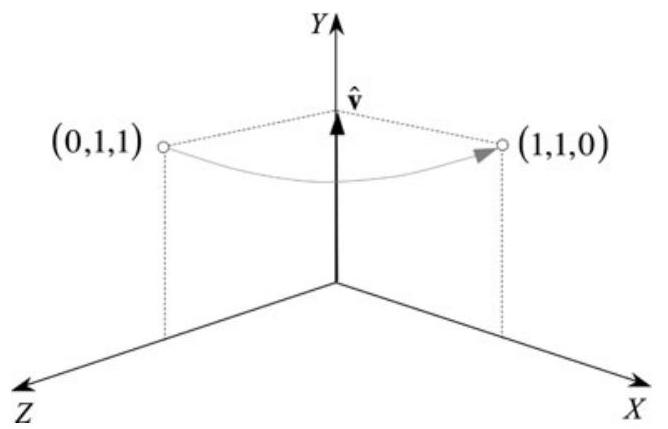
\includegraphics[max width=\textwidth]{2023_01_16_a848224efad29cd66460g-121}
\end{center}

So now we can write

$$
\begin{aligned}
q p q^{-1} & =\mathbf{R}\left(q^{-1}\right) \mathbf{L}(q) p \\
& =\left[\begin{array}{cccc}
s & x & y & z \\
-x & s & -z & y \\
-y & z & s & -x \\
-z & -y & x & s
\end{array}\right]\left[\begin{array}{cccc}
s & -x & -y & -z \\
x & s & -z & y \\
y & z & s & -x \\
z & -y & x & s
\end{array}\right]\left[\begin{array}{c}
0 \\
x_{p} \\
y_{p} \\
z_{p}
\end{array}\right] \\
& =\left[\begin{array}{cccc}
1 & 0 & 0 & 0 \\
0 & 1-2\left(y^{2}+z^{2}\right) & 2(x y-s z) & 2(x z+s y) \\
0 & 2(x y+s z) & 1-2\left(x^{2}+z^{2}\right) & 2(y z-s x) \\
0 & 2(x z-s y) & 2(y z+s x) & 1-2\left(x^{2}+y^{2}\right)
\end{array}\right]\left[\begin{array}{c}
0 \\
x_{p} \\
y_{p} \\
z_{p}
\end{array}\right] .
\end{aligned}
$$

If we ignore the first row and column, the matrix computes $\mathbf{p}^{\prime}$ :

$$
\mathbf{p}^{\prime}=\left[\begin{array}{ccc}
1-2\left(y^{2}+z^{2}\right) & 2(x y-s z) & 2(x z+s y) \\
2(x y+s z) & 1-2\left(x^{2}+z^{2}\right) & 2(y z-s x) \\
2(x z-s y) & 2(y z+s x) & 1-2\left(x^{2}+y^{2}\right)
\end{array}\right]\left[\begin{array}{l}
x_{p} \\
y_{p} \\
z_{p}
\end{array}\right]
$$

which is identical to (7.16)!

\subsection{几何验证}
Let's illustrate the action of (7.15) by rotating the point $(0,1,1), 90^{\circ}$ about the $y$ axis, as shown in Fig. 7.7. The quaternion takes the form

$$
q=\left[\cos \frac{1}{2} \theta, \sin \frac{1}{2} \theta \hat{\mathbf{v}}\right]
$$

which means that $\theta=90^{\circ}$ and $\hat{\mathbf{v}}=\mathbf{j}$, therefore,

$$
q=\left[\cos 45^{\circ}, \sin 45^{\circ} \hat{\mathbf{j}}\right]
$$

Consequently,

$$
s=\frac{\sqrt{2}}{2}, \quad x=0, \quad y=\frac{\sqrt{2}}{2}, \quad z=0 .
$$

Substituting these values in (7.15) gives

$$
\begin{aligned}
\mathbf{p}^{\prime} & =\left[\begin{array}{ccc}
2\left(s^{2}+x^{2}\right)-1 & 2(x y-s z) & 2(x z+s y) \\
2(x y+s z) & 2\left(s^{2}+y^{2}\right)-1 & 2(y z-s x) \\
2(x z-s y) & 2(y z+s x) & 2\left(s^{2}+z^{2}\right)-1
\end{array}\right]\left[\begin{array}{l}
x_{p} \\
y_{p} \\
z_{p}
\end{array}\right] \\
{\left[\begin{array}{l}
1 \\
1 \\
0
\end{array}\right] } & =\left[\begin{array}{ccc}
0 & 0 & 1 \\
0 & 1 & 0 \\
-1 & 0 & 0
\end{array}\right]\left[\begin{array}{l}
0 \\
1 \\
1
\end{array}\right]
\end{aligned}
$$

where $(0,1,1)$ is rotated to $(1,1,0)$, which is correct.

So now we have a transform that rotates a point about an arbitrary axis intersecting the origin without the problems of gimbal lock associated with Euler transforms.

Before moving on, let's evaluate one more example. Let's perform a $180^{\circ}$ rotation about a vector $\mathbf{v}=\mathbf{i}+\mathbf{k}$ passing through the origin. To begin with, we will deliberately forget to convert the vector into a unit vector, just to see what happens to the final matrix. The quaternion takes the form

$$
q=\left[\cos \frac{1}{2} \theta, \sin \frac{1}{2} \theta \hat{\mathbf{v}}\right]
$$

but we will use $\mathbf{v}$ as specified. Therefore, with $\theta=180^{\circ}$

$$
s=0, \quad x=1, \quad y=0, \quad z=1 .
$$

Substituting these values in (7.15) gives

$$
\begin{aligned}
\mathbf{p}^{\prime} & =\left[\begin{array}{ccc}
2\left(s^{2}+x^{2}\right)-1 & 2(x y-s z) & 2(x z+s y) \\
2(x y+s z) & 2\left(s^{2}+y^{2}\right)-1 & 2(y z-s x) \\
2(x z-s y) & 2(y z+s x) & 2\left(s^{2}+z^{2}\right)-1
\end{array}\right]\left[\begin{array}{l}
x_{p} \\
y_{p} \\
z_{p}
\end{array}\right] \\
& =\left[\begin{array}{ccc}
1 & 0 & 2 \\
0 & -1 & 0 \\
2 & 0 & 1
\end{array}\right]\left[\begin{array}{l}
1 \\
0 \\
0
\end{array}\right]
\end{aligned}
$$

which looks nothing like a rotation matrix, and reminds us how important it is to have a unit vector to represent the axis. Let's repeat these calculations normalising the vector to $\hat{\mathbf{v}}=\frac{1}{\sqrt{2}} \mathbf{i}+\frac{1}{\sqrt{2}} \mathbf{k}$ :

$$
s=0, \quad x=\frac{1}{\sqrt{2}}, \quad y=0, \quad z=\frac{1}{\sqrt{2}} .
$$

Substituting these values in (7.15) gives

$$
\begin{aligned}
\mathbf{p}^{\prime} & =\left[\begin{array}{ccc}
2\left(s^{2}+x^{2}\right)-1 & 2(x y-s z) & 2(x z+s y) \\
2(x y+s z) & 2\left(s^{2}+y^{2}\right)-1 & 2(y z-s x) \\
2(x z-s y) & 2(y z+s x) & 2\left(s^{2}+z^{2}\right)-1
\end{array}\right]\left[\begin{array}{l}
x_{p} \\
y_{p} \\
z_{p}
\end{array}\right] \\
{\left[\begin{array}{l}
0 \\
0 \\
1
\end{array}\right] } & =\left[\begin{array}{ccc}
0 & 0 & 1 \\
0 & -1 & 0 \\
1 & 0 & 0
\end{array}\right]\left[\begin{array}{l}
1 \\
0 \\
0
\end{array}\right]
\end{aligned}
$$

Fig. 7.8 The point $(1,0,0)$ is rotated $180^{\circ}$ about the vector $\hat{\mathbf{v}}$ to $(0,0,1)$

\begin{center}
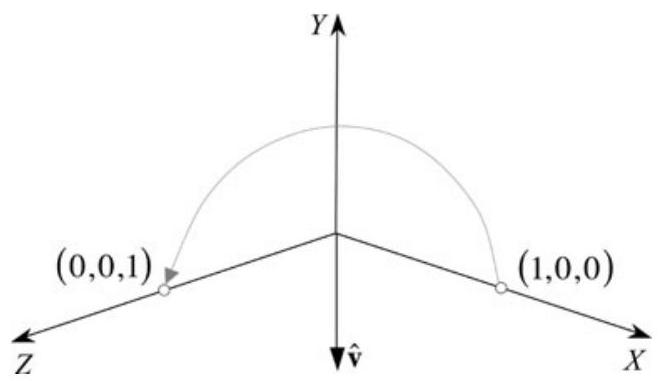
\includegraphics[max width=\textwidth]{2023_01_16_a848224efad29cd66460g-123}
\end{center}

which not only looks like a rotation matrix, but has a determinant of 1 and rotates the point $(1,0,0)$ to $(0,0,1)$ as shown in Fig. 7.8.

\section{多个旋转}
Say a vector or frame of reference is subjected to two rotations specified by $q_{1}$ followed by $q_{2}$. There is a temptation to convert both quaternions to their respective matrix and multiply the matrices together. However, this not the most efficient way of combining the rotations. It is best to accumulate the rotations as quaternions and then convert to matrix notation, if required.

To illustrate this, consider the pure quaternion $p$ subjected to the first quaternion $q_{1}$ :

$$
q_{1} p q_{1}^{-1}
$$

followed by a second quaternion $q_{2}$

$$
q_{2}\left(q_{1} p q_{1}^{-1}\right) q_{2}^{-1}
$$

which can be expressed as

$$
\left(q_{2} q_{1}\right) p\left(q_{2} q_{1}\right)^{-1} .
$$

Extra quaternions can be added accordingly. Let's illustrate this with two examples.

To keep things simple, the first quaternion $q_{1}$ rotates $30^{\circ}$ about the $y$-axis:

$$
q_{1}=\left[\cos 15^{\circ}, \sin 15^{\circ} \mathbf{j}\right] .
$$

The second quaternion $q_{2}$ rotates $60^{\circ}$ also about the $y$-axis:

$$
q_{2}=\left[\cos 30^{\circ}, \sin 30^{\circ} \mathbf{j}\right] .
$$

Together, the two quaternions rotate $90^{\circ}$ about the $y$-axis. To accumulate these rotations, we multiply them together:

$$
\begin{aligned}
q_{1} q_{2} & =\left[\cos 15^{\circ}, \sin 15^{\circ} \mathbf{j}\right]\left[\cos 30^{\circ}, \sin 30^{\circ} \mathbf{j}\right] \\
& =\left[\cos 15^{\circ} \cos 30^{\circ}-\sin 15^{\circ} \sin 30^{\circ}, \cos 15^{\circ} \sin 30^{\circ} \mathbf{j}+\cos 30^{\circ} \sin 15^{\circ} \mathbf{j}\right] \\
& =\left[\frac{\sqrt{2}}{2}, \frac{\sqrt{2}}{2} \mathbf{j}\right]
\end{aligned}
$$

which is a quaternion that rotates $90^{\circ}$ about the $y$-axis. Using the matrix (7.15) we have

$$
\begin{aligned}
\mathbf{p}^{\prime} & =\left[\begin{array}{ccc}
2\left(s^{2}+x^{2}\right)-1 & 2(x y-s z) & 2(x z+s y) \\
2(x y+s z) & 2\left(s^{2}+y^{2}\right)-1 & 2(y z-s x) \\
2(x z-s y) & 2(y z+s x) & 2\left(s^{2}+z^{2}\right)-1
\end{array}\right]\left[\begin{array}{l}
x_{p} \\
y_{p} \\
z_{p}
\end{array}\right] \\
& =\left[\begin{array}{ccc}
0 & 0 & 1 \\
0 & 1 & 0 \\
-1 & 0 & 0
\end{array}\right]\left[\begin{array}{c}
x_{p} \\
y_{p} \\
z_{p}
\end{array}\right]
\end{aligned}
$$

which rotates points about the $y$-axis by $90^{\circ}$.

For a second example, let's just evaluate the quaternions. The first quaternion $q_{1}$ rotates $90^{\circ}$ about the $x$-axis, and $q_{2}$ rotates $90^{\circ}$ about the $y$-axis:

$$
\begin{aligned}
q_{1} & =\left[\frac{\sqrt{2}}{2}, \frac{\sqrt{2}}{2} \mathbf{i}\right] \\
q_{2} & =\left[\frac{\sqrt{2}}{2}, \frac{\sqrt{2}}{2} \mathbf{j}\right] \\
p & =[0, \mathbf{i}+\mathbf{j}]
\end{aligned}
$$

therefore,

$$
\begin{aligned}
q_{2} q_{1} & =\left[\frac{\sqrt{2}}{2}, \frac{\sqrt{2}}{2} \mathbf{j}\right]\left[\frac{\sqrt{2}}{2}, \frac{\sqrt{2}}{2} \mathbf{i}\right] \\
& =\left[\frac{1}{2}, \frac{\sqrt{2}}{2} \frac{\sqrt{2}}{2} \mathbf{i}+\frac{\sqrt{2}}{2} \frac{\sqrt{2}}{2} \mathbf{j}-\frac{1}{2} \mathbf{k}\right] \\
& =\left[\frac{1}{2}, \frac{1}{2} \mathbf{i}+\frac{1}{2} \mathbf{j}-\frac{1}{2} \mathbf{k}\right] \\
\left(q_{2} q_{1}\right)^{-1} & =\left[\frac{1}{2},-\frac{1}{2} \mathbf{i}-\frac{1}{2} \mathbf{j}+\frac{1}{2} \mathbf{k}\right] \\
\left(q_{2} q_{1}\right) p & =\left[\frac{1}{2}, \frac{1}{2} \mathbf{i}+\frac{1}{2} \mathbf{j}-\frac{1}{2} \mathbf{k}\right][0, \mathbf{i}+\mathbf{j}] \\
& =\left[-\frac{1}{2}-\frac{1}{2}, \frac{1}{2}(\mathbf{i}+\mathbf{j})+\frac{1}{2} \mathbf{i}-\frac{1}{2} \mathbf{j}\right] \\
& =[-1, \mathbf{i}] \\
\left(q_{2} q_{1}\right) p\left(q_{2} q_{1}\right)^{-1} & =[-1, \mathbf{i}]\left[\frac{1}{2},-\frac{1}{2} \mathbf{i}-\frac{1}{2} \mathbf{j}+\frac{1}{2} \mathbf{k}\right] \\
& =\left[-\frac{1}{2}+\frac{1}{2}, \frac{1}{2} \mathbf{i}+\frac{1}{2} \mathbf{j}-\frac{1}{2} \mathbf{k}+\frac{1}{2} \mathbf{i}-\frac{1}{2} \mathbf{j}-\frac{1}{2} \mathbf{k}\right] \\
& =[0, \mathbf{i}-\mathbf{k}] .
\end{aligned}
$$

Thus the point $(1,1,0)$ is rotated to $(1,0,-1)$, which is correct.

\section{特征值和特征向量}
Although there is no doubt that (7.15) is a rotation matrix, we can secure further evidence by calculating its eigenvalue and eigenvector. The eigenvalue should be $\theta$ where

$$
\operatorname{Tr}\left(q p q^{-1}\right)=1+2 \cos \theta
$$

and $\operatorname{Tr}$ is the trace function, which is the sum of the diagonal elements of a matrix.

The trace of $(7.15)$ is

$$
\begin{aligned}
\operatorname{Tr}\left(q p q^{-1}\right) & =2\left(s^{2}+x^{2}\right)-1+2\left(s^{2}+y^{2}\right)-1+2\left(s^{2}+z^{2}\right)-1 \\
& =4 s^{2}+2\left(s^{2}+x^{2}+y^{2}+z^{2}\right)-3 \\
& =4 s^{2}-1 \\
& =4 \cos ^{2} \frac{1}{2} \theta-1 \\
& =4 \cos \theta+4 \sin ^{2} \frac{1}{2} \theta-1 \\
& =4 \cos \theta+2-2 \cos \theta-1 \\
& =1+2 \cos \theta
\end{aligned}
$$

and

$$
\cos \theta=\frac{1}{2}\left(\operatorname{Tr}\left(q p q^{-1}\right)-1\right) .
$$

To compute the eigenvector of (7.15) we use the three equations derived in Appendix:

$$
\begin{aligned}
& x_{v}=\left(a_{22}-1\right)\left(a_{33}-1\right)-a_{23} a_{32} \\
& y_{v}=\left(a_{33}-1\right)\left(a_{11}-1\right)-a_{31} a_{13} \\
& z_{v}=\left(a_{11}-1\right)\left(a_{22}-1\right)-a_{12} a_{21} .
\end{aligned}
$$

Therefore,

$$
\begin{aligned}
x_{v} & =\left(2\left(s^{2}+y^{2}\right)-2\right)\left(2\left(s^{2}+z^{2}\right)-2\right)-2(y z-s x) 2(y z+s x) \\
& =4\left(s^{2}+y^{2}-1\right)\left(s^{2}+z^{2}-1\right)-4\left(y^{2} z^{2}-s^{2} x^{2}\right) \\
& =4\left(\left(x^{2}+z^{2}\right)\left(x^{2}+y^{2}\right)-y^{2} z^{2}+s^{2} x^{2}\right) \\
& =4\left(x^{4}+x^{2} y^{2}+x^{2} z^{2}+z^{2} y^{2}-y^{2} z^{2}+s^{2} x^{2}\right) \\
& =4 x^{2}\left(s^{2}+x^{2}+y^{2}+z^{2}\right) \\
& =4 x^{2} .
\end{aligned}
$$

Similarly, $y_{v}=4 y^{2}$ and $z_{v}=4 z^{2}$, which confirm that the eigenvector has components associated with the quaternion's vector. The square terms should be no surprise, as the triple $q p q^{-1}$ includes the product of three quaternions. Let's test these formulae with the matrix associated with Fig. 7.8, which rotates a point $180^{\circ}$ about the vector $\hat{\mathbf{v}}=\frac{1}{\sqrt{2}} \mathbf{i}+\frac{1}{\sqrt{2}} \mathbf{k}$ :

$$
\mathbf{M}=\left[\begin{array}{lll}
a_{11} & a_{12} & a_{13} \\
a_{21} & a_{22} & a_{23} \\
a_{31} & a_{32} & a_{33}
\end{array}\right]=\left[\begin{array}{ccc}
0 & 0 & 1 \\
0 & -1 & 0 \\
1 & 0 & 0
\end{array}\right]
$$

therefore,

$$
\begin{aligned}
& x_{v}=-2 \times-1-0=2 \\
& y_{v}=-1 \times-1-1 \times 1=0 \\
& z_{v}=-1 \times-2-0=2
\end{aligned}
$$

which confirms that the eigenvector is $2 \mathbf{i}+2 \mathbf{k}$.

Next, $\operatorname{Tr}(\mathbf{M})=-1$, therefore

$$
\begin{aligned}
\cos \theta & =\frac{1}{2}\left(\operatorname{Tr}\left(q p q^{-1}\right)-1\right) \\
& =\frac{1}{2}((-1)-1) \\
& =-1 \\
\theta & =\pm 180^{\circ}
\end{aligned}
$$

which agrees with the previous results.

\section{绕偏移轴旋转}
Now that we have a matrix to represent a quaternion rotor, we can employ it to resolve problems such as rotating a point about an off-set axis using the same techniques associated with normal rotation transforms. For example, in Chap. 6 we used the following notation

$$
\left[\begin{array}{c}
x^{\prime} \\
y^{\prime} \\
z^{\prime} \\
1
\end{array}\right]=\mathbf{T}_{t_{x}, 0, t_{z}} \mathbf{R}_{\beta, y} \mathbf{T}_{-t_{x}, 0,-t_{z}}\left[\begin{array}{c}
x \\
y \\
z \\
1
\end{array}\right]
$$

to rotate a point about a fixed axis parallel with the $y$-axis. Therefore, by substituting the matrix $q p q^{-1}$ for $\mathbf{R}_{\beta, y}$ we have

$$
\left[\begin{array}{c}
x^{\prime} \\
y^{\prime} \\
z^{\prime} \\
1
\end{array}\right]=\mathbf{T}_{t_{x}, 0, t_{z}}\left(q p q^{-1}\right) \mathbf{T}_{-t_{x}, 0,-t_{z}}\left[\begin{array}{c}
x \\
y \\
z \\
1
\end{array}\right] .
$$

Let's test this by rotating our unit cube $90^{\circ}$ about the vertical axis intersecting vertices 4 and 6 as shown in Fig. 7.9. (a)

\begin{center}
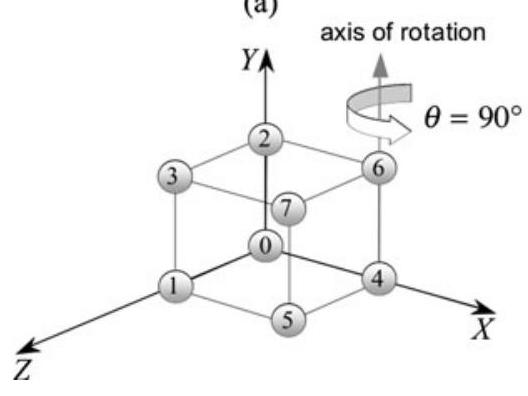
\includegraphics[max width=\textwidth]{2023_01_16_a848224efad29cd66460g-127}
\end{center}

(b)

\begin{center}
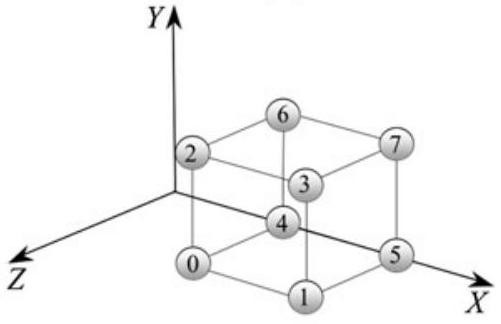
\includegraphics[max width=\textwidth]{2023_01_16_a848224efad29cd66460g-127(1)}
\end{center}

Fig. 7.9 The cube is rotated $90^{\circ}$ about the axis intersecting vertices 4 and 6

The unit-norm quaternion to achieve this is

$$
q=\left[\cos 45^{\circ}, \sin 45^{\circ} \mathbf{j}\right]
$$

with the pure quaternion

$$
p=[0, \mathbf{p}]
$$

Consequently,

$$
s=\frac{\sqrt{2}}{2}, \quad x=0, \quad y=\frac{\sqrt{2}}{2}, \quad z=0
$$

and using (7.15) in a homogeneous form we have

$$
\begin{aligned}
\mathbf{p}^{\prime} & =\left[\begin{array}{cccc}
2\left(s^{2}+x^{2}\right)-1 & 2(x y-s z) & 2(x z+s y) & 0 \\
2(x y+s z) & 2\left(s^{2}+y^{2}\right)-1 & 2(y z-s x) & 0 \\
2(x z-s y) & 2(y z+s x) & 2\left(s^{2}+z^{2}\right)-1 & 0 \\
0 & 0 & 1
\end{array}\right]\left[\begin{array}{c}
x_{p} \\
y_{p} \\
z_{p} \\
1
\end{array}\right] \\
& =\left[\begin{array}{cccc}
0 & 0 & 1 & 0 \\
0 & 1 & 0 & 0 \\
-1 & 0 & 0 & 0 \\
0 & 0 & 0 & 1
\end{array}\right]\left[\begin{array}{c}
x_{p} \\
y_{p} \\
z_{p} \\
1
\end{array}\right]
\end{aligned}
$$

The other two matrices are

$$
\begin{aligned}
\mathbf{T}_{-t_{x}, 0,0} & =\left[\begin{array}{cccc}
1 & 0 & 0 & -1 \\
0 & 1 & 0 & 0 \\
0 & 0 & 1 & 0 \\
0 & 0 & 0 & 1
\end{array}\right] \\
\mathbf{T}_{t_{x}, 0,0} & =\left[\begin{array}{llll}
1 & 0 & 0 & 1 \\
0 & 1 & 0 & 0 \\
0 & 0 & 1 & 0 \\
0 & 0 & 0 & 1
\end{array}\right] .
\end{aligned}
$$

Multiplying these three matrices together creates

$$
\left[\begin{array}{cccc}
0 & 0 & 1 & 1 \\
0 & 1 & 0 & 0 \\
-1 & 0 & 0 & 1 \\
0 & 0 & 0 & 1
\end{array}\right]
$$

Although not mathematically correct, the following statement shows the matrix (7.19) and the array of coordinates representing a unit cube, followed by the rotated cube's coordinates.

$$
\begin{gathered}
{\left[\begin{array}{cccc}
0 & 0 & 1 & 1 \\
0 & 1 & 0 & 0 \\
-1 & 0 & 0 & 1 \\
0 & 0 & 0 & 1
\end{array}\right]\left[\begin{array}{llllllll}
0 & 0 & 0 & 0 & 1 & 1 & 1 & 1 \\
0 & 0 & 1 & 1 & 0 & 0 & 1 & 1 \\
0 & 1 & 0 & 1 & 0 & 1 & 0 & 1 \\
1 & 1 & 1 & 1 & 1 & 1 & 1 & 1
\end{array}\right]} \\
=\left[\begin{array}{llllllll}
1 & 2 & 1 & 2 & 1 & 2 & 1 & 2 \\
0 & 0 & 1 & 1 & 0 & 0 & 1 & 1 \\
1 & 1 & 1 & 1 & 0 & 0 & 0 & 0 \\
1 & 1 & 1 & 1 & 1 & 1 & 1 & 1
\end{array}\right]
\end{gathered}
$$

These coordinates are confirmed by Fig. 7.9.

\section{参考系}
The product $q p q^{-1}$ is used for rotating points about the vector associated with the quaternion $q$, whereas the triple $q^{-1} p q$ can be used for rotating points about the same vector in the opposite direction. But this reverse rotation is also equivalent to a change of frame of reference. To demonstrate this, consider the problem of rotating the frame of reference $180^{\circ}$ about $\mathbf{i}+\mathbf{k}$ as shown in Fig. 7.10. The unitnorm quaternion for such a rotation is

$$
\begin{aligned}
q & =\left[\cos 90^{\circ}, \sin 90^{\circ}\left(\frac{1}{\sqrt{2}} \mathbf{i}+\frac{1}{\sqrt{2}} \mathbf{k}\right)\right] \\
& =\left[0, \frac{\sqrt{2}}{2} \mathbf{i}+\frac{\sqrt{2}}{2} \mathbf{k}\right] .
\end{aligned}
$$

Consequently,

$$
s=0, \quad x=\frac{\sqrt{2}}{2}, \quad y=0, \quad z=\frac{\sqrt{2}}{2} .
$$

Substituting these values in (7.17) we obtain

$$
\begin{aligned}
q^{-1} p q & =\left[\begin{array}{ccc}
2\left(s^{2}+x^{2}\right)-1 & 2(x y+s z) & 2(x z-s y) \\
2(x y-s z) & 2\left(s^{2}+y^{2}\right)-1 & 2(y z+s x) \\
2(x z+s y) & 2(y z-s x) & 2\left(s^{2}+z^{2}\right)-1
\end{array}\right]\left[\begin{array}{l}
x_{p} \\
y_{p} \\
z_{p}
\end{array}\right] \\
& =\left[\begin{array}{ccc}
0 & 0 & 1 \\
0 & -1 & 0 \\
1 & 0 & 0
\end{array}\right]\left[\begin{array}{l}
x_{p} \\
y_{p} \\
z_{p}
\end{array}\right]
\end{aligned}
$$

(a)

\begin{center}
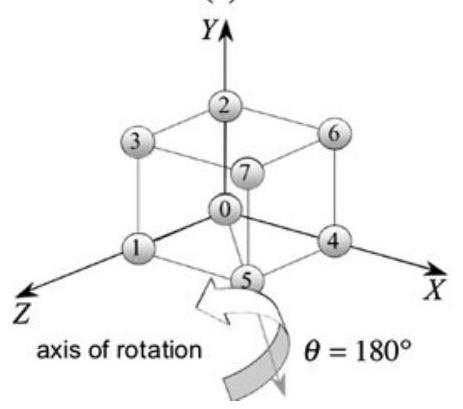
\includegraphics[max width=\textwidth]{2023_01_16_a848224efad29cd66460g-129}
\end{center}

(b)

\begin{center}
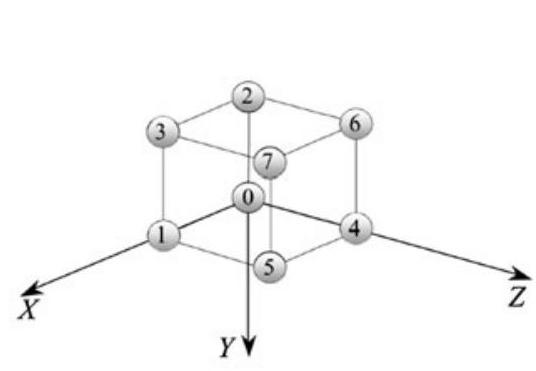
\includegraphics[max width=\textwidth]{2023_01_16_a848224efad29cd66460g-129(1)}
\end{center}

Fig. 7.10 The frame is rotated $180^{\circ}$ about the vector $\mathbf{i}+\mathbf{k}$

which, if used to process the coordinates of our unit cube, produces

$$
\begin{gathered}
{\left[\begin{array}{ccc}
0 & 0 & 1 \\
0 & -1 & 0 \\
1 & 0 & 0
\end{array}\right]\left[\begin{array}{cccccccc}
0 & 0 & 0 & 0 & 1 & 1 & 1 & 1 \\
0 & 0 & 1 & 1 & 0 & 0 & 1 & 1 \\
0 & 1 & 0 & 1 & 0 & 1 & 0 & 1
\end{array}\right]} \\
=\left[\begin{array}{cccccccc}
0 & 1 & 0 & 1 & 0 & 1 & 0 & 1 \\
0 & 0 & -1 & -1 & 0 & 0 & -1 & -1 \\
0 & 0 & 0 & 0 & 1 & 1 & 1 & 1
\end{array}\right] .
\end{gathered}
$$

This scenario is shown in Fig. $7.10$.

\section{插值四元数}
Like vectors, quaternions can be interpolated to compute an in-between quaternion. However, whereas two interpolated vectors results in a third vector that is readily visualised, two interpolated quaternions results in a third quaternion that acts as a rotor, and is not immediately visualised.

The spherical interpolant for vectors is

$$
\mathbf{v}=\frac{\sin (1-t) \theta}{\sin \theta} \mathbf{v}_{1}+\frac{\sin t \theta}{\sin \theta} \mathbf{v}_{2}
$$

where $\theta$ is the angle between the vectors, and requires no modification for quaternions:

$$
q=\frac{\sin (1-t) \theta}{\sin \theta} q_{1}+\frac{\sin t \theta}{\sin \theta} q_{2}
$$

So, given

$$
\begin{aligned}
& q_{1}=\left[s_{1}, x_{1} \mathbf{i}+y_{1} \mathbf{j}+z_{1} \mathbf{k}\right] \\
& q_{2}=\left[s_{2}, x_{2} \mathbf{i}+y_{2} \mathbf{j}+z_{2} \mathbf{k}\right]
\end{aligned}
$$

$\theta$ is obtained by taking the 4D dot product of $q_{1}$ and $q_{2}$ : Fig. 7.11 The point $(0,1,1)$ is rotated $90^{\circ}$ about the vector $\mathbf{v}_{1}$ to $(1,1,0)$
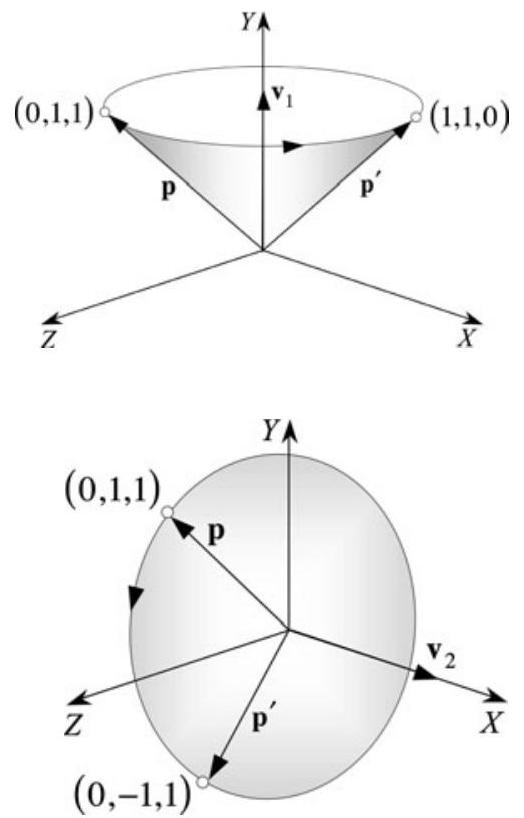
\includegraphics[max width=\textwidth, center]{2023_01_16_a848224efad29cd66460g-130}

Fig. 7.12 The point $(0,1,1)$ is rotated $90^{\circ}$ about the vector $\mathbf{v}_{2}$ to $(0,-1,1)$

$$
\begin{aligned}
\cos \theta & =\frac{q_{1} \cdot q_{2}}{\left|q_{1}\right|\left|q_{2}\right|} \\
& =\frac{s_{1} s_{2}+x_{1} x_{2}+y_{1} y_{2}+z_{1} z_{2}}{\left|q_{1}\right|\left|q_{2}\right|}
\end{aligned}
$$

and if we are working with unit-norm quaternions, then

$$
\cos \theta=s_{1} s_{2}+x_{1} x_{2}+y_{1} y_{2}+z_{1} z_{2} .
$$

Let's use (7.20) in a scenario with two simple unit-norm quaternions.

Figure $7.11$ shows one such scenario where the point $(0,1,1)$ is rotated $90^{\circ}$ about $\mathbf{v}_{1}$, the axis of $q_{1}$. Figure $7.12$ shows another scenario where the same point $(0,1,1)$ is rotated $90^{\circ}$ about $\mathbf{v}_{2}$, the axis of $q_{2}$. The quaternions are

$$
\begin{aligned}
& q_{1}=\left[\cos 45^{\circ}, \sin 45^{\circ} \mathbf{j}\right]=\left[\frac{\sqrt{2}}{2}, \frac{\sqrt{2}}{2} \mathbf{j}\right] \\
& q_{2}=\left[\cos 45^{\circ}, \sin 45^{\circ} \mathbf{i}\right]=\left[\frac{\sqrt{2}}{2}, \frac{\sqrt{2}}{2} \mathbf{i}\right] .
\end{aligned}
$$

Therefore, using (7.21)

$$
\begin{aligned}
\cos \theta & =\frac{\sqrt{2}}{2} \frac{\sqrt{2}}{2}=0.5 \\
\theta & =60^{\circ} .
\end{aligned}
$$

Before proceeding, let's compute the matrices for the two quaternion products. For $q_{1}$ :

$$
s=\frac{\sqrt{2}}{2}, \quad x=0, \quad y=\frac{\sqrt{2}}{2}, \quad z=0
$$

which when substituted in (7.15) gives

$$
\begin{aligned}
\mathbf{p}_{1}^{\prime} & =\left[\begin{array}{ccc}
2\left(s^{2}+x^{2}\right)-1 & 2(x y-s z) & 2(x z+s y) \\
2(x y+s z) & 2\left(s^{2}+y^{2}\right)-1 & 2(y z-s x) \\
2(x z-s y) & 2(y z+s x) & 2\left(s^{2}+z^{2}\right)-1
\end{array}\right]\left[\begin{array}{l}
x_{p} \\
y_{p} \\
z_{p}
\end{array}\right] \\
& =\left[\begin{array}{ccc}
0 & 0 & 1 \\
0 & 1 & 0 \\
-1 & 0 & 0
\end{array}\right]\left[\begin{array}{l}
x_{p} \\
y_{p} \\
z_{p}
\end{array}\right] .
\end{aligned}
$$

Substituting the coordinates $(0,1,1)$ in $(7.22)$ gives

$$
\left[\begin{array}{l}
1 \\
1 \\
0
\end{array}\right]=\left[\begin{array}{ccc}
0 & 0 & 1 \\
0 & 1 & 0 \\
-1 & 0 & 0
\end{array}\right]\left[\begin{array}{l}
0 \\
1 \\
1
\end{array}\right]
$$

which is correct.

For $q_{2}$ :

$$
s=\frac{\sqrt{2}}{2}, \quad x=\frac{\sqrt{2}}{2}, \quad y=0, \quad z=0
$$

which when substituted in $(7.15)$ gives

$$
\begin{aligned}
\mathbf{p}_{2}^{\prime} & =\left[\begin{array}{ccc}
2\left(s^{2}+x^{2}\right)-1 & 2(x y-s z) & 2(x z+s y) \\
2(x y+s z) & 2\left(s^{2}+y^{2}\right)-1 & 2(y z-s x) \\
2(x z-s y) & 2(y z+s x) & 2\left(s^{2}+z^{2}\right)-1
\end{array}\right]\left[\begin{array}{l}
x_{p} \\
y_{p} \\
z_{p}
\end{array}\right] \\
& =\left[\begin{array}{ccc}
1 & 0 & 0 \\
0 & 0 & -1 \\
0 & 1 & 0
\end{array}\right]\left[\begin{array}{c}
x_{p} \\
y_{p} \\
z_{p}
\end{array}\right] .
\end{aligned}
$$

Substituting the coordinates $(0,1,1)$ in $(7.23)$ gives

$$
\left[\begin{array}{c}
0 \\
-1 \\
1
\end{array}\right]=\left[\begin{array}{ccc}
1 & 0 & 0 \\
0 & 0 & -1 \\
0 & 1 & 0
\end{array}\right]\left[\begin{array}{l}
0 \\
1 \\
1
\end{array}\right]
$$

which is also correct.

Using (7.20) with $t=0.5$ computes a mid-way position for an interpolated quaternion, with its vector at $45^{\circ}$ between the $x$ - and $y$-axes, as shown in Fig. 7.13. We already know that $\theta=60^{\circ}$, therefore $\sin \theta=\sqrt{3} / 2$ :

$$
\begin{aligned}
q & =\frac{\sin (1-t) \theta}{\sin \theta} q_{1}+\frac{\sin t \theta}{\sin \theta} q_{2} \\
& =\frac{\sin \frac{1}{2} 60^{\circ}}{\sin 60^{\circ}}\left[\frac{\sqrt{2}}{2}, \frac{\sqrt{2}}{2} \mathbf{j}\right]+\frac{\sin \frac{1}{2} 60^{\circ}}{\sin 60^{\circ}}\left[\frac{\sqrt{2}}{2}, \frac{\sqrt{2}}{2} \mathbf{i}\right]
\end{aligned}
$$

Fig. 7.13 The point $(0,1,1)$ is rotated $90^{\circ}$ about the vector $\mathbf{v}$ to $(1,0,1)$

\begin{center}
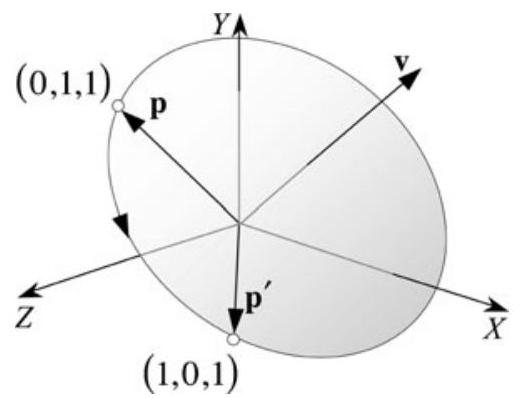
\includegraphics[max width=\textwidth]{2023_01_16_a848224efad29cd66460g-132}
\end{center}

$$
\begin{aligned}
& =\frac{1}{\sqrt{3}}\left[\frac{\sqrt{2}}{2}, \frac{\sqrt{2}}{2} \mathbf{j}\right]+\frac{1}{\sqrt{3}}\left[\frac{\sqrt{2}}{2}, \frac{\sqrt{2}}{2} \mathbf{i}\right] \\
& =\left[\frac{\sqrt{2}}{\sqrt{3}}, \frac{1}{\sqrt{6}} \mathbf{i}+\frac{1}{\sqrt{6}} \mathbf{j}\right]
\end{aligned}
$$

where

$$
s=\frac{\sqrt{2}}{\sqrt{3}}, \quad x=\frac{1}{\sqrt{6}}, \quad y=\frac{1}{\sqrt{6}}, \quad z=0
$$

which when substituted in $(7.15)$ gives

$$
\begin{aligned}
\mathbf{p}^{\prime} & =\left[\begin{array}{ccc}
2\left(s^{2}+x^{2}\right)-1 & 2(x y-s z) & 2(x z+s y) \\
2(x y+s z) & 2\left(s^{2}+y^{2}\right)-1 & 2(y z-s x) \\
2(x z-s y) & 2(y z+s x) & 2\left(s^{2}+z^{2}\right)-1
\end{array}\right]\left[\begin{array}{l}
x_{p} \\
y_{p} \\
z_{p}
\end{array}\right] \\
& =\left[\begin{array}{ccc}
\frac{2}{3} & \frac{1}{3} & \frac{2}{3} \\
\frac{1}{3} & \frac{2}{3} & -\frac{2}{3} \\
-\frac{2}{3} & \frac{2}{3} & \frac{1}{3}
\end{array}\right]\left[\begin{array}{l}
x_{p} \\
y_{p} \\
z_{p}
\end{array}\right] .
\end{aligned}
$$

Substituting the coordinates $(0,1,1)$ in $(7.24)$ gives

$$
\left[\begin{array}{l}
1 \\
0 \\
1
\end{array}\right]=\left[\begin{array}{ccc}
\frac{2}{3} & \frac{1}{3} & \frac{2}{3} \\
\frac{1}{3} & \frac{2}{3} & -\frac{2}{3} \\
-\frac{2}{3} & \frac{2}{3} & \frac{1}{3}
\end{array}\right]\left[\begin{array}{l}
0 \\
1 \\
1
\end{array}\right]
$$

which gives the point $(1,0,1)$.

One of the reasons for using a spherical interpolant is that it linearly interpolates the angle between the two unit-norm quaternions, which creates a constant-angular velocity between them. However, one of the problems with visualising quaternions is that they reside in a four-dimensional space and create a hyper-sphere with a radius equal to the quaternion's norm. With our 3D brains, this is difficult to visualise. Nevertheless, we can convince ourselves into thinking we see what is going on with a simple sketch, as shown in Fig. 7.14, where we see part of the hyper-sphere and two quaternions $q_{1}$ and $q_{2}$. In this example, the angle $\phi$ is a constant angle between two values of the interpolant $t$. The spherical interpolant also ensures that the norm Fig. 7.14 Spherical interpolation between $q_{1}$ and $q_{2}$
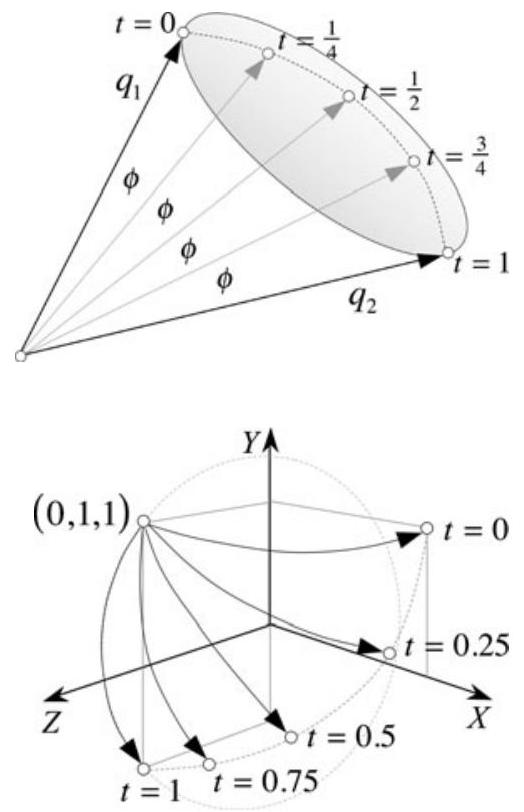
\includegraphics[max width=\textwidth, center]{2023_01_16_a848224efad29cd66460g-133}

Fig. 7.15 Sketch showing the actions of the interpolated quaternions of the interpolated quaternion remains constant at unity, preventing any unwanted scaling.

Figure $7.15$ provides another sketch to help visualise what is going on. For example, when $t=0$, the interpolated quaternion is $q_{1}$ which rotates the point $(0,1,1)$ to $(1,1,0)$, and when $t=1$, the interpolated quaternion is $q_{2}$ which rotates the point $(0,1,1)$ to $(0,-1,1)$. When $t=0.5$, the interpolated quaternion rotates the point $(0,1,1)$ to $(1,0,1)$ as computed above. Two other curves show what happens for $t=0.25$ and $t=0.75$.

A natural consequence of the interpolant is that the angle of rotation is $90^{\circ}$ for $t=0$ and $t=1$, but for $t=0.5$ the angle of rotation (eigenvalue) is approximately $70.5^{\circ}$. Corresponding angles arise for other values of $t$.

\section{将旋转矩阵转换为四元数}
The matrix transform equivalent to $q p q^{-1}$ is

$$
\begin{aligned}
q p q^{-1} & =\left[\begin{array}{ccc}
2\left(s^{2}+x^{2}\right)-1 & 2(x y-s z) & 2(x z+s y) \\
2(x y+s z) & 2\left(s^{2}+y^{2}\right)-1 & 2(y z-s x) \\
2(x z-s y) & 2(y z+s x) & 2\left(s^{2}+z^{2}\right)-1
\end{array}\right]\left[\begin{array}{l}
x_{p} \\
y_{p} \\
z_{p}
\end{array}\right] \\
& =\left[\begin{array}{lll}
a_{11} & a_{12} & a_{13} \\
a_{21} & a_{22} & a_{23} \\
a_{31} & a_{32} & a_{33}
\end{array}\right]\left[\begin{array}{l}
x_{p} \\
y_{p} \\
z_{p}
\end{array}\right] .
\end{aligned}
$$

Inspection of the matrix shows that by combining various elements we can isolate the terms of a quaternion $s, x, y, z$. For example, by adding the terms $a_{11}+a_{22}+a_{33}$ we obtain

$$
\begin{aligned}
a_{11}+a_{22}+a_{33} & =\left(2\left(s^{2}+x^{2}\right)-1\right)+\left(2\left(s^{2}+y^{2}\right)-1\right)+\left(2\left(s^{2}+z^{2}\right)-1\right) \\
& =6 s^{2}+2\left(x^{2}+y^{2}+z^{2}\right)-3 \\
& =4 s^{2}-1
\end{aligned}
$$

therefore,

$$
s=\pm \frac{1}{2} \sqrt{1+a_{11}+a_{22}+a_{33}} .
$$

To isolate $x, y$ and $z$ we employ

$$
\begin{aligned}
& x=\frac{1}{4 s}\left(a_{32}-a_{23}\right) \\
& y=\frac{1}{4 s}\left(a_{13}-a_{31}\right) \\
& z=\frac{1}{4 s}\left(a_{21}-a_{12}\right) .
\end{aligned}
$$

We can confirm their correctness using the matrix (7.25):

$$
\begin{aligned}
& \left[\begin{array}{lll}a_{11} & a_{12} & a_{13} \\a_{21} & a_{22} & a_{23} \\a_{31} & a_{32} & a_{33}\end{array}\right]=\left[\begin{array}{ccc}\frac{2}{3} & \frac{1}{3} & \frac{2}{3} \\\frac{1}{3} & \frac{2}{3} & -\frac{2}{3} \\-\frac{2}{3} & \frac{2}{3} & \frac{1}{3}\end{array}\right] \\
& s=\pm \frac{1}{2} \sqrt{1+a_{11}+a_{22}+a_{33}}=\pm \frac{1}{2} \sqrt{1+\frac{2}{3}+\frac{2}{3}+\frac{1}{3}}=\frac{\sqrt{2}}{\sqrt{3}} \\
& x=\frac{1}{4 s}\left(a_{32}-a_{23}\right)=\frac{\sqrt{3}}{4 \sqrt{2}}\left(\frac{2}{3}+\frac{2}{3}\right)=\frac{1}{\sqrt{6}} \\
& y=\frac{1}{4 s}\left(a_{13}-a_{31}\right)=\frac{\sqrt{3}}{4 \sqrt{2}}\left(\frac{2}{3}+\frac{2}{3}\right)=\frac{1}{\sqrt{6}} \\
& z=\frac{1}{4 s}\left(a_{21}-a_{12}\right)=\frac{\sqrt{3}}{4 \sqrt{2}}\left(\frac{1}{3}-\frac{1}{3}\right)=0
\end{aligned}
$$

which agree with the original values.

Say, for example, the value of $s$ had been close to zero, this could have made the values of $x, y, z$ unreliable. Consequently, other combinations are available:

$$
\begin{aligned}
& x=\pm \frac{1}{2} \sqrt{1+a_{11}-a_{22}-a_{33}} \\
& y=\frac{1}{4 x}\left(a_{12}+a_{21}\right) \\
& z=\frac{1}{4 x}\left(a_{13}+a_{31}\right)
\end{aligned}
$$

$$
\begin{aligned}
s & =\frac{1}{4 x}\left(a_{32}-a_{23}\right) \\
y & =\pm \frac{1}{2} \sqrt{1-a_{11}+a_{22}-a_{33}} \\
x & =\frac{1}{4 y}\left(a_{12}+a_{21}\right) \\
z & =\frac{1}{4 y}\left(a_{23}+a_{32}\right) \\
s & =\frac{1}{4 y}\left(a_{13}-a_{31}\right) \\
z & =\pm \frac{1}{2} \sqrt{1-a_{11}-a_{22}+a_{33}} \\
x & =\frac{1}{4 z}\left(a_{13}+a_{31}\right) \\
y & =\frac{1}{4 z}\left(a_{23}+a_{32}\right) \\
s & =\frac{1}{4 z}\left(a_{21}-a_{12}\right) .
\end{aligned}
$$

\section{欧拉角转换到四元数}
In Chap. 6 we discovered that the rotation transforms $\mathbf{R}_{\alpha, x}, \mathbf{R}_{\beta, y}$ and $\mathbf{R}_{\gamma, z}$ can be combined to create twelve triple combinations to represent a composite rotation. Now let's see how such a transform is represented by a quaternion.

To demonstrate the technique we must choose one of the twelve combinations, then the same technique can be used to convert other combinations. For example, let's choose the sequence $\mathbf{R}_{\gamma, z} \mathbf{R}_{\beta, y} \mathbf{R}_{\alpha, x}$ where the equivalent quaternions are

$$
\begin{aligned}
& q_{x}=\left[\cos \frac{1}{2} \alpha, \sin \frac{1}{2} \alpha \mathbf{i}\right] \\
& q_{y}=\left[\cos \frac{1}{2} \beta, \sin \frac{1}{2} \beta \mathbf{j}\right] \\
& q_{z}=\left[\cos \frac{1}{2} \gamma, \sin \frac{1}{2} \gamma \mathbf{k}\right]
\end{aligned}
$$

and

$$
q=q_{z} q_{y} q_{x}
$$

Expanding (7.26):

$$
\begin{aligned}
& q=\left[\cos \frac{1}{2} \gamma, \sin \frac{1}{2} \gamma \mathbf{k}\right]\left[\cos \frac{1}{2} \beta, \sin \frac{1}{2} \beta \mathbf{j}\right]\left[\cos \frac{1}{2} \alpha, \sin \frac{1}{2} \alpha \mathbf{i}\right] \\
& =\left[\cos \frac{1}{2} \gamma \cos \frac{1}{2} \beta,\right. \\
& \left.\cos \frac{1}{2} \gamma \sin \frac{1}{2} \beta \mathbf{j}+\cos \frac{1}{2} \beta \sin \frac{1}{2} \gamma \mathbf{k}-\sin \frac{1}{2} \gamma \sin \frac{1}{2} \beta \mathbf{i}\right]\left[\cos \frac{1}{2} \alpha, \sin \frac{1}{2} \alpha \mathbf{i}\right] \\
& =\left[\cos \frac{1}{2} \gamma \cos \frac{1}{2} \beta \cos \frac{1}{2} \alpha+\sin \frac{1}{2} \gamma \sin \frac{1}{2} \beta \sin \frac{1}{2} \alpha\right. \text {, } \\
& \cos \frac{1}{2} \gamma \cos \frac{1}{2} \beta \sin \frac{1}{2} \alpha \mathbf{i}+\cos \frac{1}{2} \alpha \cos \frac{1}{2} \gamma \sin \frac{1}{2} \beta \mathbf{j}+\cos \frac{1}{2} \alpha \cos \frac{1}{2} \beta \sin \frac{1}{2} \gamma \mathbf{k} \\
& \left.-\cos \frac{1}{2} \alpha \sin \frac{1}{2} \gamma \sin \frac{1}{2} \beta \mathbf{i}-\cos \frac{1}{2} \gamma \sin \frac{1}{2} \beta \sin \frac{1}{2} \alpha \mathbf{k}+\cos \frac{1}{2} \beta \sin \frac{1}{2} \gamma \sin \frac{1}{2} \alpha \mathbf{j}\right] \\
& =\left[\cos \frac{1}{2} \gamma \cos \frac{1}{2} \beta \cos \frac{1}{2} \alpha+\sin \frac{1}{2} \gamma \sin \frac{1}{2} \beta \sin \frac{1}{2} \alpha\right. \text {, } \\
& \left(\cos \frac{1}{2} \gamma \cos \frac{1}{2} \beta \sin \frac{1}{2} \alpha-\cos \frac{1}{2} \alpha \sin \frac{1}{2} \gamma \sin \frac{1}{2} \beta\right) \mathbf{i} \\
& \left(\cos \frac{1}{2} \alpha \cos \frac{1}{2} \gamma \sin \frac{1}{2} \beta+\cos \frac{1}{2} \beta \sin \frac{1}{2} \gamma \sin \frac{1}{2} \alpha\right) \mathbf{j} \\
& \left.\left(\cos \frac{1}{2} \alpha \cos \frac{1}{2} \beta \sin \frac{1}{2} \gamma-\cos \frac{1}{2} \gamma \sin \frac{1}{2} \beta \sin \frac{1}{2} \alpha\right) \mathbf{k}\right] \text {. }
\end{aligned}
$$

Now let's place the angles in a consistent sequence:

$$
\begin{aligned}
s & =\cos \frac{1}{2} \gamma \cos \frac{1}{2} \beta \cos \frac{1}{2} \alpha+\sin \frac{1}{2} \gamma \sin \frac{1}{2} \beta \sin \frac{1}{2} \alpha \\
x_{q} & =\cos \frac{1}{2} \gamma \cos \frac{1}{2} \beta \sin \frac{1}{2} \alpha-\sin \frac{1}{2} \gamma \sin \frac{1}{2} \beta \cos \frac{1}{2} \alpha \\
y_{q} & =\cos \frac{1}{2} \gamma \sin \frac{1}{2} \beta \cos \frac{1}{2} \alpha+\sin \frac{1}{2} \gamma \cos \frac{1}{2} \beta \sin \frac{1}{2} \alpha \\
z_{q} & =\sin \frac{1}{2} \gamma \cos \frac{1}{2} \beta \cos \frac{1}{2} \alpha-\cos \frac{1}{2} \gamma \sin \frac{1}{2} \beta \sin \frac{1}{2} \alpha
\end{aligned}
$$

where

$$
q=\left[s, x_{q} \mathbf{i}+y_{q} \mathbf{j}+z_{q} \mathbf{k}\right] .
$$

Let's test (7.27). We start with the three rotation transforms

$$
\begin{aligned}
\mathbf{R}_{\alpha, x} & =\left[\begin{array}{ccc}
1 & 0 & 0 \\
0 & \cos \alpha & -\sin \alpha \\
0 & \sin \alpha & \cos \alpha
\end{array}\right] \\
\mathbf{R}_{\beta, y} & =\left[\begin{array}{ccc}
\cos \beta & 0 & \sin \beta \\
0 & 1 & 0 \\
-\sin \beta & 0 & \cos \beta
\end{array}\right]
\end{aligned}
$$

$$
\mathbf{R}_{\gamma, z}=\left[\begin{array}{ccc}
\cos \gamma & -\sin \gamma & 0 \\
\sin \gamma & \cos \gamma & 0 \\
0 & 0 & 1
\end{array}\right]
$$

Then

$$
\begin{aligned}
& \mathbf{R}_{\gamma, z} \mathbf{R}_{\beta, y} \mathbf{R}_{\alpha, x} \\
&= {\left[\begin{array}{ccc}
\cos \gamma \cos \beta & -\sin \gamma \cos \alpha+\cos \gamma \sin \beta \sin \alpha & \sin \gamma \sin \alpha+\cos \gamma \sin \beta \cos \alpha \\
\sin \gamma \cos \beta & \cos \gamma \cos \alpha+\sin \gamma \sin \beta \sin \alpha & -\cos \gamma \sin \alpha+\sin \gamma \sin \beta \cos \alpha \\
-\sin \beta & \cos \beta \sin \alpha & \cos \beta \cos \alpha
\end{array}\right] . }
\end{aligned}
$$

Let's make $\alpha=\beta=\gamma=90^{\circ}$, then

$$
\mathbf{R}_{90^{\circ}, z} \mathbf{R}_{90^{\circ}, y} \mathbf{R}_{90^{\circ}, x}=\left[\begin{array}{ccc}
0 & 0 & 1 \\
0 & 1 & 0 \\
-1 & 0 & 0
\end{array}\right]
$$

which rotates points $90^{\circ}$ about the $y$-axis:

$$
\left[\begin{array}{l}
1 \\
1 \\
0
\end{array}\right]=\left[\begin{array}{ccc}
0 & 0 & 1 \\
0 & 1 & 0 \\
-1 & 0 & 0
\end{array}\right]\left[\begin{array}{l}
0 \\
1 \\
1
\end{array}\right]
$$

Now let's evaluate (7.27):

$$
\begin{aligned}
s & =\cos \frac{1}{2} \gamma \cos \frac{1}{2} \beta \cos \frac{1}{2} \alpha+\sin \frac{1}{2} \gamma \sin \frac{1}{2} \beta \sin \frac{1}{2} \alpha \\
& =\frac{\sqrt{2}}{2} \frac{\sqrt{2}}{2} \frac{\sqrt{2}}{2}+\frac{\sqrt{2}}{2} \frac{\sqrt{2}}{2} \frac{\sqrt{2}}{2} \\
& =\frac{\sqrt{2}}{2} \\
x_{q} & =\cos \frac{1}{2} \gamma \cos \frac{1}{2} \beta \sin \frac{1}{2} \alpha-\sin \frac{1}{2} \gamma \sin \frac{1}{2} \beta \cos \frac{1}{2} \alpha \\
& =0 \\
y_{q} & =\cos \frac{1}{2} \gamma \sin \frac{1}{2} \beta \cos \frac{1}{2} \alpha+\sin \frac{1}{2} \gamma \cos \frac{1}{2} \beta \sin \frac{1}{2} \alpha \\
& =\frac{\sqrt{2}}{2} \frac{\sqrt{2}}{2} \frac{\sqrt{2}}{2}+\frac{\sqrt{2}}{2} \frac{\sqrt{2}}{2} \frac{\sqrt{2}}{2} \\
& =\frac{\sqrt{2}}{2} \\
z_{q} & =\sin \frac{1}{2} \gamma \cos \frac{1}{2} \beta \cos \frac{1}{2} \alpha-\cos \frac{1}{2} \gamma \sin \frac{1}{2} \beta \sin \frac{1}{2} \alpha \\
& =0
\end{aligned}
$$

and

$$
q=\left[\frac{\sqrt{2}}{2}, \frac{\sqrt{2}}{2} \mathbf{j}\right]
$$

which is a quaternion that also rotates points $90^{\circ}$ about the $y$-axis.

\section{总结}
This chapter has been the focal point of the book where unit-norm quaternions have been used to rotate a vector about a quaternion's vector. It would have been useful if this could have been achieved by the simple product $q p$, like complex numbers. But as we saw, this only works when the quaternion is orthogonal to the vector. The product $q p q^{-1}$ —discovered by Hamilton and Cayley-works for all orientations between a quaternion and a vector. It is also relatively easy to compute. We also saw that the product can be represented as a matrix, which can be integrated with other matrices.

Perhaps one of the most interesting features of quaternions that has emerged in this chapter, is that their imaginary qualities are not required in any calculations, because they are embedded within the algebra.

The spherical interpolant provides a clever way to dynamically change a quaternion's axis and angle of rotation, but can be difficult to visualise as an animated sequence without access to a real-time display system.

The reverse product $q^{-1} p q$ reverses the angle of rotation, and is equivalent to changing the sign of the rotation angle in $q p q^{-1}$. Consequently, it can be used to rotate a frame of reference in the same direction as $q p q^{-1}$.

\subsection{操作符总结}
\subsubsection*{Rotating a point about a vector}
$$
\begin{aligned}
q & =[s, \mathbf{v}] \\
s^{2}+|\mathbf{v}|^{2} & =1 \\
p & =[0, \mathbf{p}] \\
q p q^{-1} & =\left[0,2(\mathbf{v} \cdot \mathbf{p}) \mathbf{v}+\left(2 s^{2}-1\right) \mathbf{p}+2 s \mathbf{v} \times \mathbf{p}\right] \\
q & =\left[\cos \frac{1}{2} \theta, \sin \frac{1}{2} \theta \hat{\mathbf{v}}\right] \\
p & =[0, \mathbf{p}] \\
q p q^{-1} & =[0,(1-\cos \theta)(\hat{\mathbf{v}} \cdot \mathbf{p}) \hat{\mathbf{v}}+\cos \theta \mathbf{p}+\sin \theta \hat{\mathbf{v}} \times \mathbf{p}]
\end{aligned}
$$

\subsubsection*{Rotating a frame about a vector}
$$
q^{-1} p q=[0,(1-\cos \theta)(\hat{\mathbf{v}} \cdot \mathbf{p}) \hat{\mathbf{v}}+\cos \theta \mathbf{p}-\sin \theta \hat{\mathbf{v}} \times \mathbf{p}]
$$

\subsubsection*{Matrix for rotating a point about a vector}
$$
\mathbf{p}^{\prime}=\left[\begin{array}{ccc}
1-2\left(y^{2}+z^{2}\right) & 2(x y-s z) & 2(x z+s y) \\
2(x y+s z) & 1-2\left(x^{2}+z^{2}\right) & 2(y z-s x) \\
2(x z-s y) & 2(y z+s x) & 1-2\left(x^{2}+y^{2}\right)
\end{array}\right]\left[\begin{array}{c}
x_{p} \\
y_{p} \\
z_{p}
\end{array}\right]
$$

\subsubsection*{Matrix for rotating a frame about a vector}
$$
\mathbf{p}^{\prime}=\left[\begin{array}{ccc}
1-2\left(y^{2}+z^{2}\right) & 2(x y+s z) & 2(x z-s y) \\
2(x y-s z) & 1-2\left(x^{2}+z^{2}\right) & 2(y z+s x) \\
2(x z+s y) & 2(y z-s x) & 1-2\left(x^{2}+y^{2}\right)
\end{array}\right]\left[\begin{array}{l}
x_{p} \\
y_{p} \\
z_{p}
\end{array}\right]
$$

\subsubsection*{Matrix for a quaternion product}
$$
\begin{aligned}
& q_{1} q_{2}=\mathbf{L}\left(q_{1}\right) q_{2}= {\left[\begin{array}{cccc}
s_{1} & -x_{1} & -y_{1} & -z_{1} \\
x_{1} & s_{1} & -z_{1} & y_{1} \\
y_{1} & z_{1} & s_{1} & -x_{1} \\
z_{1} & -y_{1} & x_{1} & s_{1}
\end{array}\right]\left[\begin{array}{l}
s_{2} \\
x_{2} \\
y_{2} \\
z_{2}
\end{array}\right] } \\
& q_{1} q_{2}=\mathbf{R}\left(q_{2}\right) q_{1}=\left[\begin{array}{cccc}
s_{2} & -x_{2} & -y_{2} & -z_{2} \\
x_{2} & s_{2} & z_{2} & -y_{2} \\
y_{2} & -z_{2} & s_{2} & x_{2} \\
z_{2} & y_{2} & -x_{2} & s_{2}
\end{array}\right]\left[\begin{array}{l}
s_{1} \\
x_{1} \\
y_{1} \\
z_{1}
\end{array}\right]
\end{aligned}
$$

\subsubsection*{Interpolating two quaternions}
$$
q=\frac{\sin (1-t) \theta}{\sin \theta} q_{1}+\frac{\sin t \theta}{\sin \theta} q_{2}
$$

where

$$
\begin{aligned}
\cos \theta & =\frac{q_{1} \cdot q_{2}}{\left|q_{1}\right|\left|q_{2}\right|} \\
& =\frac{s_{1} s_{2}+x_{1} x_{2}+y_{1} y_{2}+z_{1} z_{2}}{\left|q_{1}\right|\left|q_{2}\right|}
\end{aligned}
$$

\subsubsection*{Quaternion from a rotation matrix}
$$
\begin{aligned}
& s=\pm \frac{1}{2} \sqrt{1+a_{11}+a_{22}+a_{33}} \\
& x=\frac{1}{4 s}\left(a_{32}-a_{23}\right) \\
& y=\frac{1}{4 s}\left(a_{13}-a_{31}\right) \\
& z=\frac{1}{4 s}\left(a_{21}-a_{12}\right) \\
& x=\pm \frac{1}{2} \sqrt{1+a_{11}-a_{22}-a_{33}} \\
& y=\frac{1}{4 x}\left(a_{12}+a_{21}\right) \\
& z=\frac{1}{4 x}\left(a_{13}+a_{31}\right) \\
& s=\frac{1}{4 x}\left(a_{32}-a_{23}\right) \\
& y=\pm \frac{1}{2} \sqrt{1-a_{11}+a_{22}-a_{33}}
\end{aligned}
$$

$$
\begin{aligned}
x & =\frac{1}{4 y}\left(a_{12}+a_{21}\right) \\
z & =\frac{1}{4 y}\left(a_{23}+a_{32}\right) \\
s & =\frac{1}{4 y}\left(a_{13}-a_{31}\right) \\
z & =\pm \frac{1}{2} \sqrt{1-a_{11}-a_{22}+a_{33}} \\
x & =\frac{1}{4 z}\left(a_{13}+a_{31}\right) \\
y & =\frac{1}{4 z}\left(a_{23}+a_{32}\right) \\
s & =\frac{1}{4 z}\left(a_{21}-a_{12}\right)
\end{aligned}
$$

\subsubsection*{Eigenvector and eigenvalue}
$$
\begin{aligned}
x_{v} & =\left(a_{22}-1\right)\left(a_{33}-1\right)-a_{23} a_{32} \\
y_{v} & =\left(a_{33}-1\right)\left(a_{11}-1\right)-a_{31} a_{13} \\
z_{v} & =\left(a_{11}-1\right)\left(a_{22}-1\right)-a_{12} a_{21} \\
\cos \theta & =\frac{1}{2}\left(\operatorname{Tr}\left(q p q^{-1}\right)-1\right)
\end{aligned}
$$

\subsubsection*{Euler angles to quaternion}
Using the transform $\mathbf{R}_{\gamma, z} \mathbf{R}_{\beta, y} \mathbf{R}_{\alpha, x}$ :

$$
\begin{aligned}
s & =\cos \frac{1}{2} \gamma \cos \frac{1}{2} \beta \cos \frac{1}{2} \alpha+\sin \frac{1}{2} \gamma \sin \frac{1}{2} \beta \sin \frac{1}{2} \alpha \\
x_{q} & =\cos \frac{1}{2} \gamma \cos \frac{1}{2} \beta \sin \frac{1}{2} \alpha-\sin \frac{1}{2} \gamma \sin \frac{1}{2} \beta \cos \frac{1}{2} \alpha \\
y_{q} & =\cos \frac{1}{2} \gamma \sin \frac{1}{2} \beta \cos \frac{1}{2} \alpha+\sin \frac{1}{2} \gamma \cos \frac{1}{2} \beta \sin \frac{1}{2} \alpha \\
z_{q} & =\sin \frac{1}{2} \gamma \cos \frac{1}{2} \beta \cos \frac{1}{2} \alpha-\cos \frac{1}{2} \gamma \sin \frac{1}{2} \beta \sin \frac{1}{2} \alpha
\end{aligned}
$$

where

$$
q=\left[s, x_{q} \mathbf{i}+y_{q} \mathbf{j}+z_{q} \mathbf{k}\right]
$$

\section{样例}
Here are some further worked examples that employ the ideas described above.

Example 1 Use $q p$ to rotate $p=[0, \mathbf{j}] 90^{\circ}$ about the $x$-axis.

For this to work $q$ must be orthogonal to $p$ :

$$
\begin{aligned}
q & =[\cos \theta, \sin \theta \mathbf{i}] \\
& =[0, \mathbf{i}]
\end{aligned}
$$

and

$$
\begin{aligned}
p^{\prime} & =q p \\
& =[0, \mathbf{i}][0, \mathbf{j}] \\
& =[0, \mathbf{k}] .
\end{aligned}
$$

Example 2 Use $q p q^{-1}$ to rotate $p=[0, \mathbf{j}] 90^{\circ}$ about the $x$-axis.

For this to work:

$$
\begin{aligned}
q & =\left[\cos \frac{1}{2} \theta, \sin \frac{1}{2} \theta \mathbf{i}\right] \\
& =\left[\frac{\sqrt{2}}{2}, \frac{\sqrt{2}}{2} \mathbf{i}\right]
\end{aligned}
$$

and

$$
\begin{aligned}
p^{\prime} & =q p q^{-1} \\
& =\left[\frac{\sqrt{2}}{2}, \frac{\sqrt{2}}{2} \mathbf{i}\right][0, \mathbf{j}]\left[\frac{\sqrt{2}}{2},-\frac{\sqrt{2}}{2} \mathbf{i}\right] \\
& =\left[0, \frac{\sqrt{2}}{2} \mathbf{j}+\frac{\sqrt{2}}{2} \mathbf{k}\right]\left[\frac{\sqrt{2}}{2},-\frac{\sqrt{2}}{2} \mathbf{i}\right] \\
& =\left[0, \frac{\sqrt{2}}{2}\left(\frac{\sqrt{2}}{2} \mathbf{j}+\frac{\sqrt{2}}{2} \mathbf{k}\right)+\frac{1}{2} \mathbf{j}+\frac{1}{2} \mathbf{k}\right] \\
& =\left[0, \frac{1}{2} \mathbf{j}+\frac{1}{2} \mathbf{k}-\frac{1}{2} \mathbf{j}+\frac{1}{2} \mathbf{k}\right] \\
& =[0, \mathbf{k}]
\end{aligned}
$$

which agrees with the answer for Example 1.

Example 3 Evaluate the triple $q p q^{-1}$ for $p=[0, \mathbf{p}]$ and $q=\left[\cos \frac{1}{2} \theta, \sin \frac{1}{2} \theta \mathbf{v}\right]$, where $\theta=360^{\circ}$.

$$
\begin{aligned}
q & =[-1, \mathbf{0}] \\
q p q^{-1} & =[-1, \mathbf{0}][0, \mathbf{p}][-1, \mathbf{0}] \\
& =[0,-\mathbf{p}][-1, \mathbf{0}] \\
& =[0, \mathbf{p}]
\end{aligned}
$$

which confirms that the vector remains unmoved, as expected.

Example 4 Compute the matrix (7.15) for $q=\left[\frac{1}{2}, \frac{\sqrt{3}}{2} \mathbf{k}\right]$, and find its eigenvector and eigenvalue. From $q$

$$
\begin{aligned}
& s=\frac{1}{2}, \quad x=0, \quad y=0, \quad z=\frac{\sqrt{3}}{2} \\
& \mathbf{p}^{\prime}=\left[\begin{array}{ccc}2\left(s^{2}+x^{2}\right)-1 & 2(x y-s z) & 2(x z+s y) \\2(x y+s z) & 2\left(s^{2}+y^{2}\right)-1 & 2(y z-s x) \\2(x z-s y) & 2(y z+s x) & 2\left(s^{2}+z^{2}\right)-1\end{array}\right]\left[\begin{array}{l}x_{p} \\y_{p} \\z_{p}\end{array}\right] \\
& =\left[\begin{array}{ccc}-\frac{1}{2} & -\frac{\sqrt{3}}{2} & 0 \\\frac{\sqrt{3}}{2} & -\frac{1}{2} & 0 \\0 & 0 & 1\end{array}\right]\left[\begin{array}{l}x_{p} \\y_{p} \\z_{p}\end{array}\right] \text {. }
\end{aligned}
$$

If we plug in the point $(1,0,0)$ it is rotated about the $z$-axis by $120^{\circ}$ :

$$
\left[\begin{array}{c}
-\frac{1}{2} \\
\frac{\sqrt{3}}{2} \\
1
\end{array}\right]=\left[\begin{array}{ccc}
-\frac{1}{2} & -\frac{\sqrt{3}}{2} & 0 \\
\frac{\sqrt{3}}{2} & -\frac{1}{2} & 0 \\
0 & 0 & 1
\end{array}\right]\left[\begin{array}{l}
1 \\
0 \\
0
\end{array}\right]
$$

Using

$$
\begin{aligned}
\cos \theta & =\frac{1}{2}\left(\operatorname{Tr}\left(q p q^{-1}\right)-1\right) \\
& =\frac{1}{2}(0-1) \\
\theta & =120^{\circ}
\end{aligned}
$$

Using

$$
\begin{aligned}
x_{v} & =\left(a_{22}-1\right)\left(a_{33}-1\right)-a_{23} a_{32} \\
& =\left(-\frac{3}{2}\right)(0)-0 \\
& =0 \\
y_{v} & =\left(a_{33}-1\right)\left(a_{11}-1\right)-a_{31} a_{13} \\
& =(0)\left(-\frac{3}{2}\right)-0 \\
& =0 \\
z_{v} & =\left(a_{11}-1\right)\left(a_{22}-1\right)-a_{12} a_{21} \\
& =\left(-\frac{3}{2}\right)\left(-\frac{3}{2}\right)+\frac{\sqrt{3}}{2} \frac{\sqrt{3}}{2} \\
& =3
\end{aligned}
$$

which makes the eigenvector $3 \mathbf{k}$ and the eigenvalue $120^{\circ}$. Example 5 Find the half-way quaternion between $q_{1}=\left[\cos \frac{1}{2} \alpha, \sin \frac{1}{2} \alpha \mathbf{k}\right]$ and $q_{2}=$ $\left[\cos \frac{1}{2} \alpha, \sin \frac{1}{2} \alpha \mathbf{i}\right]$ when $\alpha=90^{\circ}$. Show that it is a unit-norm quaternion, and find its angle of rotation.

The angle between $q_{1}$ and $q_{2}$ is $\theta$ where

$$
\begin{aligned}
\cos \theta & =\frac{s_{1} s_{2}+x_{1} x_{2}+y_{1} y_{2}+z_{1} z_{2}}{\left|q_{1}\right|\left|q_{2}\right|} \\
& =\cos ^{2} \frac{1}{2} \alpha \\
& =0.5 \\
\theta & =60^{\circ} .
\end{aligned}
$$

Using

$$
\begin{aligned}
q & =\frac{\sin (1-t) \theta}{\sin \theta} q_{1}+\frac{\sin t \theta}{\sin \theta} q_{2} \\
& =\frac{\sin 30^{\circ}}{\sin 60^{\circ}}\left[\cos 45^{\circ}, \sin 45^{\circ} \mathbf{k}\right]+\frac{\sin 30^{\circ}}{\sin 60^{\circ}}\left[\cos 45^{\circ}, \sin 45^{\circ} \mathbf{i}\right] \\
& =\frac{1}{\sqrt{3}}\left[\frac{\sqrt{2}}{2}, \frac{\sqrt{2}}{2} \mathbf{k}\right]+\frac{1}{\sqrt{3}}\left[\frac{\sqrt{2}}{2}, \frac{\sqrt{2}}{2} \mathbf{i}\right] \\
& =\left[\frac{\sqrt{2}}{\sqrt{3}}, \frac{\sqrt{2}}{2 \sqrt{3}} \mathbf{i}+\frac{\sqrt{2}}{2 \sqrt{3}} \mathbf{k}\right] \\
& =\left[\frac{2}{\sqrt{6}}, \frac{1}{\sqrt{6}} \mathbf{i}+\frac{1}{\sqrt{6}} \mathbf{k}\right]
\end{aligned}
$$

The norm of $q$ is

$$
\begin{aligned}
|q| & =\left(\frac{2}{\sqrt{6}}\right)^{2}+\left(\frac{1}{\sqrt{6}}\right)^{2}+\left(\frac{1}{\sqrt{6}}\right)^{2} \\
& =\frac{2}{3}+\frac{1}{6}+\frac{1}{6} \\
& =1
\end{aligned}
$$

Therefore, $\cos \frac{1}{2} \alpha=\frac{\sqrt{2}}{\sqrt{3}}$ and $\sin \frac{1}{2} \alpha=\frac{1}{\sqrt{3}}$, and $\alpha \approx 70.5^{\circ}$.

Example 6 Convert the given matrix into a quaternion and identify its function.

$$
\mathbf{M}=\left[\begin{array}{ccc}
0 & 0 & 1 \\
0 & 1 & 0 \\
-1 & 0 & 0
\end{array}\right]
$$

therefore,

$$
\begin{aligned}
s & =\frac{1}{2} \sqrt{1+a_{11}+a_{22}+a_{33}} \\
& =\frac{1}{2} \sqrt{1+0+1+0}=\frac{\sqrt{2}}{2}
\end{aligned}
$$

$$
\begin{aligned}
x & =\frac{1}{4 s}\left(a_{32}-a_{23}\right) \\
& =\frac{\sqrt{2}}{4}(0+0)=0 \\
y & =\frac{1}{4 s}\left(a_{13}-a_{31}\right) \\
& =\frac{\sqrt{2}}{4}(1+1)=\frac{\sqrt{2}}{2} \\
z & =\frac{1}{4 s}\left(a_{21}-a_{12}\right) \\
& =\frac{\sqrt{2}}{4}(0+0)=0
\end{aligned}
$$

which is the quaternion $\left[\frac{\sqrt{2}}{2}, \frac{\sqrt{2}}{2} \mathbf{j}\right]$ which is a rotation of $90^{\circ}$ about the $y$-axis.
